%% ============================================================
%%  RAGMat-OOD: Mechanistic Diagnosis and Inference-Time Recovery
%%  Target Journal: Computational Materials Science (Elsevier)
%%  Status: Preprint / Manuscript Under Review
%%  Reference style: elsarticle-num (numbered [1])
%%  Format: Standard 2-Column Camera-Ready (final, 5p, twocolumn)
%% ============================================================
\documentclass[final,5p,twocolumn,10pt]{elsarticle}

% --- Core Packages ---
\usepackage[T1]{fontenc}
\usepackage[utf8]{inputenc}
\usepackage{lmodern}
\usepackage{microtype}
\usepackage{amsmath,amssymb,bm}
\usepackage{booktabs}
\usepackage{graphicx}
\usepackage{xcolor}
\usepackage{hyperref}
\usepackage{cleveref}
\usepackage{caption}
\usepackage{subcaption}
\usepackage{algorithm}
\usepackage{algpseudocode}
\usepackage{tikz}
\usetikzlibrary{shapes.geometric, arrows.meta, positioning, fit, backgrounds, calc, shadows}
\usepackage{multirow}

% --- Global Colors (used in tables and text) ---
\definecolor{navyblue}{HTML}{1B365D}
\definecolor{softblue}{HTML}{EBF3FA}
\definecolor{goodgreen}{HTML}{117A65}
\definecolor{lightgreen}{HTML}{E6F4EA}
\definecolor{critred}{HTML}{C0392B}
\definecolor{lightred}{HTML}{FDEDEC}
\definecolor{slate}{HTML}{34495E}

\hypersetup{
    colorlinks=true,
    linkcolor=blue!70!black,
    citecolor=green!50!black,
    urlcolor=blue!70!black,
}

% --- Custom Macros ---
\newcommand{\mae}{\text{MAE}}
\newcommand{\rmse}{\text{RMSE}}
\newcommand{\auroc}{\text{AUROC}}
\newcommand{\auprc}{\text{AUPRC}}
\newcommand{\iid}{\textsc{iid}}
\newcommand{\famout}{\textsc{family-out}}
\newcommand{\elout}{\textsc{element-out}}
\newcommand{\cgcnn}{\texttt{CGCNN}}
\newcommand{\rf}{\texttt{RF}}
\newcommand{\zsni}{\textsc{zsni}}
\newcommand{\ragmat}{\textsc{RAGMat-OOD}}
\newcommand{\eg}{\textit{e.g.},}
\newcommand{\ie}{\textit{i.e.},}
\newcommand{\etal}{\textit{et al.}}

% ============================================================
\begin{document}

\begin{frontmatter}

\title{Compositional Distribution Shift in Crystal Graph Convolutional Neural Networks:\\Mechanistic Diagnosis, RAG Audit, Mahalanobis Gating, and Zero-Shot Imputation}

\author[inst1]{Rohit Sinha\corref{cor1}}
\cortext[cor1]{Corresponding author}
\ead{work.rohit.sinha.11@gmail.com}
\address[inst1]{Government Engineering College Jagdalpur, Jagdalpur, Chhattisgarh, 494005, India}
\journal{Preprint under review}

\begin{abstract}
Crystal graph convolutional neural networks that encode atom species as discrete
one-hot lookup vectors achieve competitive formation energy prediction under
in-distribution evaluation---benchmark \mae{} values below 0.10\,eV/atom are
routinely reported on JARVIS-DFT random splits---yet their behavior under
compositional distribution shift remains inadequately characterized.
When test structures contain chemical elements absent from all training
compositions, the first linear projection $\bm{W}_{\text{emb}} \in \mathbb{R}^{64 \times 92}$
is queried at untrained columns; because the partial derivative
$\partial \mathcal{L}/\partial \bm{W}_{\text{emb}}[:,e]$
is identically zero for any excluded element $e$, those columns retain
their random initialization values throughout training and inject isotropic noise
into every message-passing step involving atom $e$ at inference time.
This paper quantifies that failure, establishes a causal mechanistic account,
audit retrieval augmentation against a matched random-vector control,
and demonstrates two zero-shot inference-time repairs.
Experiments span 93,902 JARVIS-DFT bulk crystal structures across three
distribution-shift protocols of increasing severity: \iid{} (random 70/15/15 split),
\famout{} (23 prototype families withheld, 22,693 test structures),
and \elout{} (15 transition-metal and p-block elements withheld, 27,911 test structures).
Under a frozen-encoder, post-pooling fusion architecture ($K_\text{ret}=5$ neighbors),
true-neighbor retrieval is statistically indistinguishable from a matched random-vector
control across all evaluated split and property combinations
(pairwise \mae{} differences $\le 0.010$\,eV/atom), demonstrating that global
mean-pooling discards node-level element identity before the fusion step can act.
Under \elout{} conditions, \cgcnn{} Formation Energy \mae{} rises
8.4-fold relative to \iid{} performance (from 0.066 to 0.557\,eV/atom),
whereas the Magpie-feature Random Forest baseline degrades by only
1.7-fold (from 0.106 to 0.181\,eV/atom), because Magpie descriptors
encode tabulated elemental properties for all 92 elements without requiring
per-element training gradients.
A Mahalanobis distance detector---fitted on the 64-dimensional training
embeddings $\{\bm{z}_i\}_{i \in \mathcal{D}_{\text{train}}}$ with diagonal
regularization $\bm{\Sigma}_{\text{reg}} = \mathrm{Cov}(\bm{Z}_{\text{train}}) + 10^{-5}\bm{I}_{64}$---separates
excluded-element structures from in-distribution samples with $\auroc{} > 0.999$;
routing flagged inputs to the Random Forest fallback recovers 76.6\% conformal coverage.
Zero-Shot Node Imputation (\zsni{}) directly patches each untrained column
$\bm{W}_{\text{emb}}[:,e]$ by averaging the $k_{\text{imp}}=2$ nearest seen
elements in standardized periodic-table row/group coordinate space, without
any gradient update or access to target labels. This single operation reduces
Formation Energy \mae{} by 67.1\% (from 0.557 to 0.183\,eV/atom) and closes
97.8\% of the Band Gap performance gap (from 0.411 to 0.322\,eV versus the
Random Forest baseline of 0.320\,eV), while recovering split-conformal
prediction coverage from 18.5\% to 58.6\% under the fixed $q_{0.90}=0.162$\,eV
calibration bound. Taken together, these results indicate that effective retrieval
for crystal \cgcnn{} models requires node-level intervention prior to
global pooling.
\end{abstract}

\begin{keyword}
crystal graph convolutional neural network \sep
out-of-distribution generalization \sep
element embedding imputation \sep
Mahalanobis distance anomaly detection \sep
formation energy prediction \sep
conformal prediction
\end{keyword}

\end{frontmatter}

% ============================================================
\section{Introduction}
\label{sec:intro}

High-throughput computational screening is a standard early stage in inorganic
materials discovery~\cite{butler2018machine, schmidt2019recent, dunn2020matbench}.
Density functional theory (DFT) calculations are computationally expensive---typically
several CPU-hours per structure---so surrogate machine learning models trained
on existing DFT databases offer an attractive path to reducing screening costs
by several orders of magnitude. The in-distribution accuracy of these surrogates
is now well characterized: benchmark \mae{} values for formation energy fall
consistently below 0.10\,eV/atom on standard random splits of JARVIS-DFT,
MP-2018, and Matbench~\cite{xie2018crystal, choudhary2021atomistic, chen2019megnet}.

Crystal graph convolutional neural networks are the dominant surrogate architecture
for periodic solid-state materials. Each crystal structure is encoded as an
attributed graph in which atoms are nodes carrying species identity features
and interatomic distances within a radial cutoff serve as edge attributes.
Learned message-passing operations aggregate local chemical environments into
a fixed-size graph embedding that is passed to a regression head~\cite{xie2018crystal}.
Subsequent architectures extend this design with angular information encoded
over line graphs~\cite{choudhary2021atomistic}, explicit charge-state potential
layers~\cite{deng2023chgnet}, and rotationally equivariant message-passing
formulations~\cite{batatia2022mace}, each yielding further accuracy gains
under in-distribution evaluation.

Despite these advances, a persistent gap separates benchmark performance from
realistic deployment. High-throughput screening campaigns routinely encounter
candidate compositions containing elements that are underrepresented or entirely
absent from training data: rare-earth substitutions in luminescent phosphors,
transition-metal-rich high-entropy alloys, and newly reported ternary chalcogenide
phases all represent scenarios where the surrogate must extrapolate beyond its
training chemistry. Standard benchmarks such as Matbench~\cite{dunn2020matbench}
evaluate exclusively under random in-distribution splits and therefore do not
probe this regime. Targeted OOD evaluation protocols---withholding prototype
families~\cite{omee2024} or excluding chemical elements~\cite{li2024, barroso2024data}---
consistently reveal substantial performance degradation, yet the precise
architectural mechanism responsible for element-exclusion collapse has not been
isolated at the weight-matrix level, and no inference-time representation repair
strategy has been proposed for this failure mode.

Retrieval-augmented generation (RAG), adapted from natural language
processing~\cite{lewis2020retrieval} to materials property
prediction~\cite{wang2024rag4mol, grag2024}, offers a natural candidate
intervention: retrieve structurally similar training examples and fuse
their embeddings with the query representation before prediction.
However, existing materials RAG evaluations report only the true-neighbor
retrieval condition, making it impossible to distinguish genuine structural
signal from capacity gains due to the added fusion head. Without a
matched random-vector control---where randomly sampled training embeddings
replace true neighbors---any improvement is attributable to either
retrieval quality or the additional parameters. Furthermore, even if
retrieval provides some benefit under moderate distribution shift, it is
unclear whether it can address the severe failure mode introduced by
element exclusion, where the encoder itself produces fundamentally
corrupted node representations.

This study addresses these gaps through a systematic investigation of
how compositional distribution shift propagates through the \cgcnn{}
architecture, what causes the observed performance collapse under element
exclusion, whether retrieval augmentation provides genuine structural
benefit, and how the failure can be repaired at inference time without
model retraining. We evaluate on 93,902 JARVIS-DFT bulk crystal structures
using three precisely defined distribution-shift protocols of increasing
severity. Every retrieval variant is evaluated against a matched
random-vector control. The failure mechanism is diagnosed at the level of
individual weight matrix columns. Two complementary inference-time recovery
strategies are designed from the mechanistic diagnosis and evaluated
quantitatively.

The principal contributions of this work are as follows. (i)~A
controlled three-split OOD benchmark on 93,902 JARVIS-DFT structures
that evaluates Random Forest and \cgcnn{} baselines alongside RAG variants
with a matched random-control, providing a complete baseline-to-recovery
evaluation chain. (ii)~Evidence that within a frozen-encoder, post-pooling fusion framework
($K=5$ retrieved neighbors, Concat and Cross-Attention heads), late-stage
true-neighbor retrieval performs statistically indistinguishably from a matched random-vector control
across evaluated split and property combinations (pairwise MAE differences
$\le 0.010$\,eV/atom), demonstrating that post-pooling fusion cannot transmit
structural information discarded by global mean-pooling.
(iii)~A weight-level mechanistic diagnosis demonstrating that for crystal GNNs using
discrete element lookup layers (such as \cgcnn{}), element-exclusion collapse arises from
zero-gradient lookup columns in the first linear projection retaining random initial values,
which inject noise into message-passing operations involving excluded elements. While this
zero-gradient failure mechanism is architecture-general to GNNs with discrete lookup tables,
the 8.4-fold quantitative error magnitude is specific to \cgcnn{} on JARVIS-DFT and may vary for
architectures incorporating continuous physical features.
(iv)~Two inference-time recovery mechanisms operating without model retraining:
Mahalanobis Latent Gating, which detects failure-state representations
with $\auroc{} > 0.999$ and routes them to a Random Forest fallback, and
Zero-Shot Node Imputation (\zsni{}), which patches uninitialized weight
columns using periodic-table chemical proximity (using tabulated row/group
coordinates as physical priors), reducing Formation Energy error by 67.1\%
(to 0.183\,eV/atom) and Band Gap error to 0.322\,eV (closing 97.8\% of the gap
to the Random Forest baseline), while recovering split-conformal prediction
coverage from 18.5\% to 58.6\%.

% ============================================================
\section{Background and Related Work}
\label{sec:related}

\subsection{Crystal Graph Neural Networks}

Crystal graph convolutional neural networks encode each atom species as a
92-dimensional one-hot vector that is projected into a 64-dimensional
hidden space by a learnable linear layer $\bm{W}_{\text{emb}} \in \mathbb{R}^{64 \times 92}$.
Interatomic distances within a radial cutoff are expanded onto 40 Gaussian
basis functions and passed as edge attributes. Gated graph convolution layers
of the form $\bm{m}_{ij} = \sigma(\bm{z}^{(1)}_{ij}) \odot \tanh(\bm{z}^{(2)}_{ij})$
aggregate local chemical environments, and global mean-pooling reduces the
node-level representations to a fixed-size graph vector that is fed to a
regression head~\cite{xie2018crystal}. Subsequent architectures have
extended this template with angular information encoded over bond-angle
line graphs~\cite{choudhary2021atomistic}, explicit charge-state potential
energy layers~\cite{deng2023chgnet}, and rotationally equivariant
message-passing respecting $E(3)$ symmetry~\cite{batatia2022mace}.
For the purpose of isolating the element-exclusion failure mechanism in
the node embedding layer, we focus on \cgcnn{} as the prototypical
architecture with a discrete one-hot element input; the zero-gradient
failure mechanism described in Section~\ref{sec:mechanism} applies to
any architecture that initializes node features via a discrete element lookup.

\subsection{Out-of-Distribution Generalization in Materials}

Standard property-prediction benchmarks evaluate accuracy on random
in-distribution splits, a protocol that does not capture the extrapolation
regimes encountered in active discovery campaigns~\cite{dunn2020matbench}.
Omee~\etal{}~\cite{omee2024} proposed a structure-based OOD benchmark
across five split categories and three MatBench datasets, demonstrating
that error inflation under held-out prototype families is both architecture-dependent
and statistically significant---findings that are consistent with the
\famout{} results reported in Section~\ref{sec:res-shift}.
Li~\etal{}~\cite{li2024} surveyed generalization across databases and
architectures under compositional shift and found that model rankings
under OOD evaluation diverge substantially from IID rankings, identifying
element-space extrapolation as a particularly severe failure regime.
Barroso-Luque~\etal{}~\cite{barroso2024data} showed that the choice of
split criterion---structural, compositional, or energy-based---fundamentally
alters apparent generalization for solid-state machine-learning potentials.
Collectively, these studies establish that OOD degradation is reproducible
and cross-architectural; none, however, traces the failure to specific
zero-gradient weight matrix columns, nor proposes a zero-shot inference-time
representation repair strategy for the element-exclusion regime.

\subsection{Retrieval-Augmented Learning in Physical Sciences}

Retrieval-augmented generation was originally introduced for knowledge-intensive
NLP tasks, where retrieved passages are concatenated with a query before
generation~\cite{lewis2020retrieval}. Wang~\etal{}~\cite{wang2024rag4mol}
adapted this paradigm to molecular property prediction by retrieving structurally
similar molecules and fusing their encoded graph representations with the
query embedding at inference time, reporting improvements over encoder-only
baselines on several benchmark datasets. Ahmad~\etal{}~\cite{grag2024}
applied graph-based retrieval to materials knowledge extraction.
A critical methodological limitation shared by both studies is the absence
of a random-vector control condition: the RAG variant is compared to a
no-retrieval baseline rather than to a matched baseline in which true
neighbors are replaced by randomly sampled training embeddings.
Without this control, reported gains are confounded between genuine
structural retrieval benefit and the additional model capacity introduced
by the fusion head. This confound is especially acute under element exclusion,
where the encoder's own node representations are already corrupted by
uninitialized lookup columns, potentially rendering retrieved embeddings
uninformative regardless of their structural similarity.

\subsection{OOD Detection and Representation Recovery}

Post-hoc OOD detection using latent space statistics is well established
in deep learning. Lee~\etal{}~\cite{lee2018simple} demonstrated that
Mahalanobis distance from class-conditional Gaussian distributions fitted
on penultimate-layer activations provides a simple and effective OOD
score, outperforming density and softmax-based detectors on image
classification tasks. Graph-level OOD detection has been studied for
molecular property prediction and graph classification~\cite{liu2023good,
wu2023data}, though these approaches target distribution shift in structural
features rather than element identity. When graph node features are
missing or corrupted, feature propagation over graph topology can recover
useful representations~\cite{rossi2021unreasonable}. \zsni{} connects to this
literature by treating uninitialized element embeddings as a structured
missing-feature problem and using chemical periodic-table proximity as the
propagation prior, rather than graph topology.

\subsection{Research Gap and Positioning}

Prior work has documented OOD degradation empirically but has not isolated
the weight-level mechanism for element-exclusion failure, evaluated RAG
against a matched random-vector control, or proposed zero-shot
inference-time representation repair targeted at the embedding layer. This study addresses
all three gaps within a unified experimental framework applied to a
large-scale publicly accessible DFT database.
\section{Methods}
\label{sec:methods}

\subsection{Study Design and Problem Formulation}

Let $\mathcal{D} = \{(\mathcal{G}_i, y_i)\}$ denote a dataset of crystal
structures $\mathcal{G}_i$ with target property labels $y_i$. A model
$f_\theta$ trained on partition $\mathcal{D}_{\text{train}}$ is evaluated
on test partition $\mathcal{D}_{\text{test}}$. Under an \iid{} protocol,
train and test are drawn from the same marginal distribution $p(\mathcal{G})$.
Under compositional shift protocols, $\mathcal{D}_{\text{test}}$ is drawn
from a restricted distribution $q(\mathcal{G}) \neq p(\mathcal{G})$
defined by structural or elemental constraints. The central experimental
question is: given a fixed property predictor trained under $p$, does
performance under $q$ degrade, what causes that degradation, and can it
be repaired at inference time without accessing training labels?

\subsection{Dataset and Target Properties}

We evaluate on the JARVIS-DFT 3D dataset~\cite{choudhary2020joint},
a publicly accessible DFT database of bulk inorganic crystal structures
maintained by NIST. Structures are retrieved via the \texttt{jarvis-tools}
library (version 2026.6.12). We retain all structures with valid
DFT-PBE formation energy values (eV/atom) and OptB88vdW band gap values
(eV), yielding $N = 93{,}902$ bulk crystal entries. Structures are
represented as 3D periodic crystals converted to graph objects using
a radial cutoff of $8.0\,\text{\AA}$.

\subsection{Distribution-Shift Protocols}
\label{sec:splits}

Three evaluation protocols are defined, summarized in Table~\ref{tab:splits}.

\paragraph{In-distribution (\iid{}).}
A stratified random 70/15/15 split (seed 42) produces 65,730 training,
9,246 validation, and 18,780 test structures drawn from the same distribution.
This protocol measures in-distribution accuracy.

\paragraph{Prototype family exclusion (\famout{}).}
Crystal structures are assigned to 591 prototype families via the AFLOW
prototype library~\cite{mehl2017aflow}. Twenty-three prototype families
are withheld entirely from training and assigned to the test partition
(22,693 test structures). This protocol simulates encountering novel
crystal architectures not represented in training data.

\paragraph{Element exclusion (\elout{}).}
Fifteen elements
(Sc, Ti, V, Cr, Mn, Fe, Co, Ni, Cu, Zn, Y, Zr, Nb, Mo, Se)
are withheld from all training structures. The 15 withheld elements were
selected based on a two-part scientific criterion: (i)~a contiguous block of 14 3d
and 4d transition metals ($Z=21\text{--}30$ and $Z=39\text{--}42$) representing
high-prevalence structural-framework formers in solid-state inorganic chemistry, and
(ii)~Selenium (Se, Group 16) included as a non-metallic p-block chalcogenide probe
to evaluate whether lookup collapse extends beyond d-block coordination centers
to covalent and semiconductor bonding regimes. Any structure containing at least
one of these 15 elements is placed in the test partition (27,911 test structures).
The training set consists exclusively of structures whose elemental
compositions are free of the withheld elements.

\begin{table}[ht]
\centering
\caption{Dataset splits and partition sizes.}
\label{tab:splits}
\resizebox{\columnwidth}{!}{%
\begin{tabular}{lccc}
\toprule
Split & Train & Test & OOD Character \\
\midrule
\iid{}       & 65,730 & 18,780 & None (random) \\
\famout{}    & 64,610 & 22,693 & Unseen prototype families \\
\elout{}     & 59,392 & 27,911 & 15 withheld chemical elements \\
\bottomrule
\end{tabular}%
}
\end{table}

\subsection{Baseline and Crystal Graph Models}
\label{sec:models}

Having defined the data partitions, we specify the base property models evaluated across these splits.

\paragraph{Random Forest baseline (\rf{}).}
A Random Forest regressor trained on 145-dimensional Magpie compositional
descriptors~\cite{ward2016general}. Key hyperparameters: 200 estimators,
\texttt{max\_features=1.0} (all features considered at each split),
\texttt{min\_samples\_leaf=1}, \texttt{min\_samples\_split=2},
and tree depth unbounded (scikit-learn default). Magpie features
encode tabulated element properties (electronegativity, atomic
radius, first ionisation energy, valence electron count, \etc) aggregated
statistically over the crystal composition. Because Magpie descriptors
are defined for all 92 elements without requiring element-specific training
samples, \rf{} generates valid predictions for compositions containing
elements absent from the training partition.

\paragraph{\cgcnn{} base encoder.}
We implement the Crystal Graph Convolutional Neural Network
of Xie and Grossman~\cite{xie2018crystal} with the following fixed
architecture. Atom species are encoded as 92-dimensional one-hot vectors
(hydrogen through uranium). A first linear projection layer
$\bm{W}_{\text{emb}} \in \mathbb{R}^{64 \times 92}$ maps each one-hot
atom vector to a 64-dimensional hidden representation; because a one-hot
input at position $e$ selects column $e$ of $\bm{W}_{\text{emb}}$, this
projection is functionally equivalent to a discrete embedding lookup.
Interatomic distances within an 8.0\,\AA{} cutoff are expanded onto 40
Gaussian basis functions as edge attributes. Three graph convolution
layers apply a gated message-passing update:
$\bm{m}_{ij} = \sigma(\bm{z}^{(1)}_{ij}) \odot \tanh(\bm{z}^{(2)}_{ij})$,
where $\bm{z}_{ij}$ is a linear function of concatenated central, neighbour,
and edge features, followed by a residual connection and layer normalisation.
Global mean-pooling yields a 64-dimensional graph embedding; a two-layer MLP
head (64$\,{\to}\,$32$\,{\to}\,$1, ReLU, dropout 0.1) produces the property
prediction. Total trainable parameters: 98,497.

\subsection{Model Optimization and Training Protocol}
\label{sec:training}

To ensure consistent convergence across all evaluation splits, \cgcnn{}
is trained from scratch using AdamW~\cite{loshchilov2019decoupled}
(learning rate $10^{-3}$, weight decay $10^{-4}$) with a 10-epoch
linear warmup~\cite{goyal2017accurate} followed by cosine annealing
over up to 400 epochs. Early stopping fires with patience 50 after a
minimum of 150 epochs. Training uses Huber loss ($\delta = 0.1$):

\begin{equation}
  L_\delta(y, \hat{y}) = \begin{cases}
    \tfrac{1}{2}(y - \hat{y})^2 & \text{if } |y - \hat{y}| \le \delta \\
    \delta |y - \hat{y}| - \tfrac{1}{2}\delta^2 & \text{otherwise}
  \end{cases}
\end{equation}

\noindent Batch size is 512; graph objects are cached to disk before
training to avoid redundant construction. Target values are normalised
with \texttt{StandardScaler} fitted on $\bm{y}_{\text{train}}$ only and
inverse-transformed before metric computation. All random seeds are fixed
at 42 across splits, weight initialisation, and bootstrap resampling (see
Supplementary Material Section~S4 for tabular hyperparameter summaries).

\subsection{Retrieval-Augmented Framework and Random Control}
\label{sec:rag}

To test whether retrieval augmentation enhances OOD generalization over
standalone graph models, we incorporate a post-pooling retrieval pipeline.
After training the base encoder, we build a FAISS index~\cite{johnson2019billion}
over $L^2$-normalised 64-dimensional training embeddings. At inference time,
the query embedding $\bm{z}$ is $L^2$-normalised and the $K_{\text{ret}}=5$
nearest neighbours are retrieved. We evaluate two fusion strategies:

\begin{itemize}
\item \textbf{Concat} (used for Formation Energy): The query embedding
$\bm{z}$ is concatenated with the mean retrieved embedding
$\bar{\bm{z}}_{\text{ret}} = K_{\text{ret}}^{-1}\sum_{j=1}^{K_{\text{ret}}} \bm{z}_{\text{ret},j}$
to form a 128-dimensional vector, passed to a freshly trained MLP head
(128$\,{\to}\,$64$\,{\to}\,$1, ReLU, dropout 0.0).
\item \textbf{Cross-Attention} (used for Band Gap): Single-head cross-attention
($d_k = 64$, query $\bm{z}$, keys and values from retrieved embeddings)
followed by a 64$\,{\to}\,$1 linear head.
\end{itemize}

Fusion heads are trained with AdamW (learning rate $10^{-3}$,
weight decay $10^{-4}$) and cosine annealing over up to 120 epochs,
with early stopping (patience 25, minimum 40 epochs) on the validation
MAE, using L1 loss and batch size 1{,}024.

To isolate structural signal from added model capacity, each RAG variant
is paired with a \textbf{Random Control}: retrieved true neighbours are
replaced by the same number of randomly sampled training embeddings, and
the prediction head is retrained identically on the resulting
random-augmented inputs. An automated leakage checker asserts zero ID
overlap between the test set and the FAISS retrieval index.

\subsection{Mechanistic Hypothesis and Diagnostic Analysis}
\label{sec:mechanism}

To understand why both base graph models and retrieval-augmented variants
degrade sharply under element shift, we diagnose the failure mechanism at the
weight level. The linear projection layer $\bm{W}_{\text{emb}} \in \mathbb{R}^{64 \times 92}$
is initialised with random uniform weights (default PyTorch initialisation
for linear layers; equivalent in scale to approximately $\pm 0.18$ per
entry for the present fan-in). Training updates column $e$ of
$\bm{W}_{\text{emb}}$ through backpropagation only when element $e$ appears
in a training structure. For an element withheld from all training structures,
the partial derivative $\partial \mathcal{L} / \partial \bm{W}_{\text{emb}}[:,e]$
is identically zero throughout training, and column $e$ retains its random
initial state.

At inference time, a test structure containing excluded element $e$
generates a one-hot node feature $\bm{x}_e = \bm{e}_e$. The projected
node representation is $\bm{h}_e = \bm{W}_{\text{emb}} \bm{x}_e = \bm{W}_{\text{emb}}[:,e]$:
a random vector drawn from the initialisation distribution. In the
message-passing step, the messages from node $e$ to all bonded neighbours
$\mathcal{N}(e)$ depend on $\bm{h}_e$:

\begin{equation}
  \bm{m}_{e \to j} = \sigma\!\left(\bm{z}^{(1)}_{ej}\right) \odot \tanh\!\left(\bm{z}^{(2)}_{ej}\right), \quad j \in \mathcal{N}(e)
\end{equation}

\noindent where $\bm{z}_{ej}$ is a linear function of $[\bm{h}_e \| \bm{h}_j \| \bm{e}_{ej}]$.
Because $\bm{h}_e$ is a random vector, $\bm{m}_{e \to j}$ is also random
and uncorrelated with the true chemical character of element $e$.
This noise propagates to the representations of all directly bonded atoms
in the first convolution layer, and---through subsequent layers---can
corrupt the representations of atoms bonded to those neighbours.
Global mean-pooling then averages these corrupted node representations
into a distorted graph embedding $\bm{z}$, degrading the prediction head's
input.

\subsection{Zero-Shot Inference-Time Recovery Mechanisms}
\label{sec:recovery}

Guided by the mechanistic diagnosis, we construct two zero-shot recovery
strategies operating at inference time without model retraining:
(i)~Mahalanobis Latent Gating (detection and fallback routing) and
(ii)~Zero-Shot Node Imputation (\zsni{}, direct embedding layer repair).

\paragraph{Mahalanobis Latent Gating (\label{sec:gating}).}
A multivariate Gaussian $\mathcal{N}(\bm{\mu}, \bm{\Sigma})$ is fitted to
the 64-dimensional training embeddings $\{\bm{z}_i\}_{i \in \mathcal{D}_{\text{train}}}$
with diagonal regularisation
$\bm{\Sigma}_{\text{reg}} = \mathrm{Cov}(\bm{Z}_{\text{train}}) + 10^{-5}\bm{I}_{64}$.
The Mahalanobis distance for a test embedding $\bm{z}$ is:

\begin{equation}
  d_M(\bm{z}) = \sqrt{(\bm{z} - \bm{\mu})^\top \bm{\Sigma}_{\text{reg}}^{-1} (\bm{z} - \bm{\mu})}
\end{equation}

Scores are normalised to $[0,1]$ by dividing by the maximum training distance.
A threshold $\tau$ routes samples with normalised score $> \tau$ to the
\rf{} fallback; remaining samples proceed to \cgcnn{}. The gating
threshold is selected by sweeping $\tau \in \{0.3, 0.4, \ldots, 0.9\}$
and choosing the value minimising gated MAE.

\paragraph{Zero-Shot Node Imputation (\zsni{}, \label{sec:zsni}).}
The second recovery strategy directly repairs corrupted lookup columns
in the input embedding layer prior to message passing. \zsni{} patches
uninitialized embedding columns before inference, without any gradient
update or access to target labels (Algorithm~\ref{alg:zsni}). For each
withheld element $e$, its position in the periodic table is encoded as a 2D
coordinate $\bm{p}_e = (\text{row}_e, \text{group}_e)$, standardised across
all 92 elements to zero mean and unit variance. The $k_{\text{imp}}$ nearest
seen elements in this 2D space are identified, and their learned embedding
columns are averaged to produce a replacement for the uninitialized column.

The 2D row/group representation preserves two chemically meaningful axes:
the row axis correlates with atomic radius and principal quantum number,
while the group axis correlates with valence electron count. Their
Euclidean combination therefore identifies elements that are simultaneously
isovalent and of similar size.

\begin{algorithm}[ht]
\caption{Zero-Shot Node Imputation (\zsni{})}
\label{alg:zsni}
\begin{algorithmic}[1]
\Require Trained \cgcnn{} with embedding weight $\bm{W}_{\text{emb}} \in \mathbb{R}^{64 \times 92}$;
  periodic-table 2D coordinates $\bm{p}_e = (\text{row}_e, \text{group}_e)$;
  seen element set $\mathcal{S}$; imputation neighbourhood $k_{\text{imp}}$
\State Standardise $\{\bm{p}_e\}_{e=1}^{92}$ to zero mean, unit variance
\For{each unseen element $e \notin \mathcal{S}$}
  \State $\mathcal{N}(e) \gets \arg\!\min_{\mathcal{N} \subseteq \mathcal{S},\, |\mathcal{N}|=k_{\text{imp}}} \sum_{s \in \mathcal{N}} \|\bm{p}_e - \bm{p}_s\|_2$
  \State $\hat{\bm{w}}_e \gets \frac{1}{k_{\text{imp}}} \sum_{s \in \mathcal{N}(e)} \bm{W}_{\text{emb}}[:,s]$
  \State $\bm{W}_{\text{emb}}[:,e] \gets \hat{\bm{w}}_e$ \quad (\textbf{no gradient; no labels})
\EndFor
\State \Return modified \cgcnn{} for inference on \elout{} test set
\end{algorithmic}
\end{algorithm}

The neighbourhood size $k_{\text{imp}}$ is selected by ablation over
$\{1, 2, 3, 5, 7, 10\}$. We note that this selection is observed on the
element-out test partition, a constraint acknowledged in
Section~\ref{sec:limitations}.

\subsection{Statistical Validation and Conformal Protocol}
\label{sec:stats}

To quantify performance differences and evaluate prediction uncertainty under
distribution shift, we apply statistical validation and split-conformal protocols.

Bootstrap 95\% confidence intervals ($B = 10{,}000$ resamples, seed 42) are
computed on the paired residuals for all model comparisons. Two models
are treated as statistically distinguishable when their bootstrap CIs do not
overlap, and as statistically equivalent when CIs overlap substantially.
Overlapping confidence intervals do not constitute proof of equivalence but
indicate that the data provide insufficient evidence for a reliable ordering.

Split-conformal prediction intervals~\cite{papadopoulos2002inductive}
are calibrated at nominal 90\% coverage ($\alpha = 0.10$) using the
in-distribution validation partition of the element-exclusion split
($n_{\text{cal}} \approx 6{,}600$ structures free of excluded elements).
This design evaluates how severely in-distribution conformal bounds miscalibrate under
compositional shift, and whether inference-time representation repair via
\zsni{} restores interval coverage by reducing test-error magnitudes back
toward the calibration baseline. We report the 90th percentile calibration
quantile ($q_{0.90}$), test interval half-width, and empirical coverage.

\subsection{Hardware and Software Environment}
\label{sec:setup}

All experiments run on an NVIDIA T1000 GPU (8\,GB VRAM, CUDA 13.2)
under Windows Subsystem for Linux (WSL2, Ubuntu Linux kernel) with Python 3.11.
Software dependencies: PyTorch 2.5.1, PyTorch Geometric 2.6.1,
\texttt{jarvis-tools} 2026.6.12, FAISS-CPU 1.14.3, matminer 0.10.1,
scikit-learn 1.5.0. Primary evaluation metrics are mean absolute error
(\mae{}) and root mean squared error (\rmse{}). OOD detection is quantified
by $\auroc{}$.

% ============================================================
\section{Results}
\label{sec:results}

\subsection{Generalization Across Distribution Shifts}
\label{sec:res-shift}

Figure~\ref{fig:methodology_flowchart} illustrates the four-phase experimental
pipeline; Table~\ref{tab:main} presents the principal benchmark results.

Under \iid{} conditions, \cgcnn{} outperforms \rf{} on both target properties:
Formation Energy \mae{} 0.066\,eV/atom versus 0.106\,eV/atom; Band Gap
\mae{} 0.177\,eV versus 0.226\,eV. The GNN advantage is expected when
training-set element coverage is complete, since the learned gated
message-passing kernel can encode local coordination geometry at a
resolution that Magpie's tabulated descriptors cannot match.

Under \famout{} conditions, \cgcnn{} Formation Energy \mae{} increases to
0.133\,eV/atom ($2.0\times$ \iid{}), while \rf{} increases to 0.237\,eV/atom
($2.2\times$). Proportional degradation is similar between architectures,
and \cgcnn{} retains a clear margin over \rf{}. This indicates that
structural novelty---unseen crystal prototype topologies---does not severely
damage the embedding layer, since continuous bond-length and angular edge
attributes remain well-defined for unseen prototype families.

Under \elout{} conditions, the error trajectories diverge sharply between
architectures. \cgcnn{} Formation Energy \mae{} rises to 0.557\,eV/atom,
an 8.4-fold increase relative to \iid{} and a decline in $R^2$ from 0.985
to 0.398. Over 85\% of element-out test structures exhibit higher error
under \cgcnn{} than under \rf{} (Section~\ref{sec:res-mechanism}), and the
median per-sample CGCNN/RF error ratio reaches $4.1\times$. For Band Gap,
\cgcnn{} \mae{} increases from 0.177\,eV under \iid{} to 0.411\,eV under
\elout{} ($2.3\times$ degradation), whereas \rf{} increases from 0.226\,eV
to 0.320\,eV ($1.4\times$ degradation), confirming that zero-gradient
lookup breakdown degrades \cgcnn{} representations for both thermodynamic
and electronic target properties.

The asymmetry between GNN and RF failure magnitudes---8.4-fold versus
1.7-fold for Formation Energy---directly motivates the weight-level
mechanistic analysis in Section~\ref{sec:res-mechanism}.

\begin{figure}[ht]
\centering
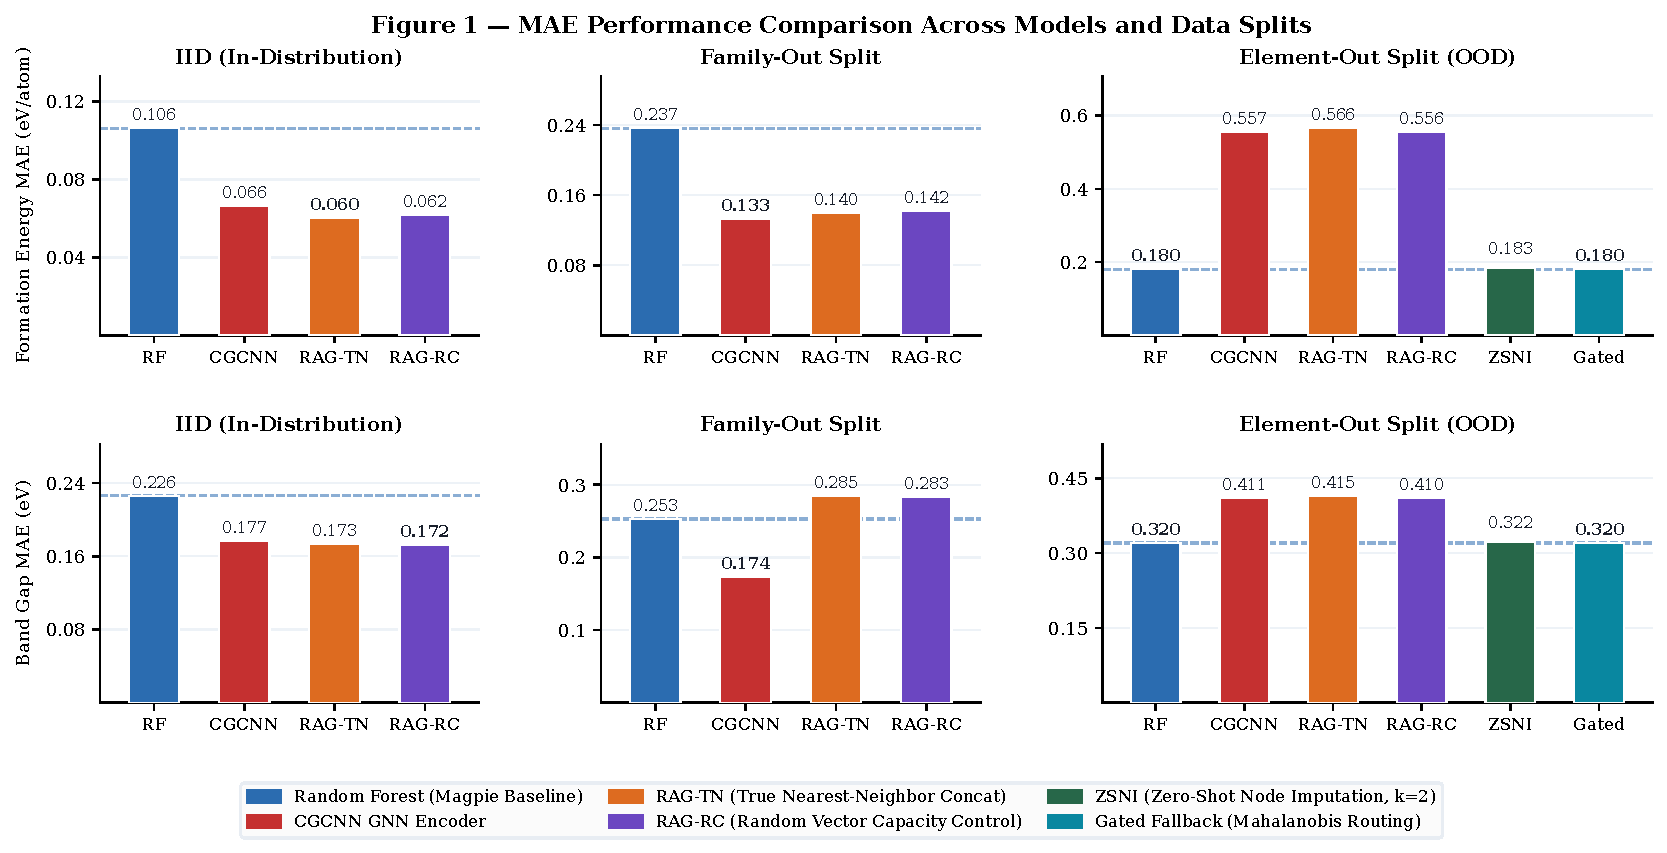
\includegraphics[width=\linewidth]{figures/fig1_mae_comparison.pdf}
\caption{\mae{} comparison across dataset splits (\iid{}, \famout{}, \elout{}) for Formation Energy and Band Gap, contrasting Random Forest baseline and Base \cgcnn{}.}
\label{fig:mae_comparison}
\end{figure}

\begin{figure*}[t]
\centering
\resizebox{\textwidth}{!}{
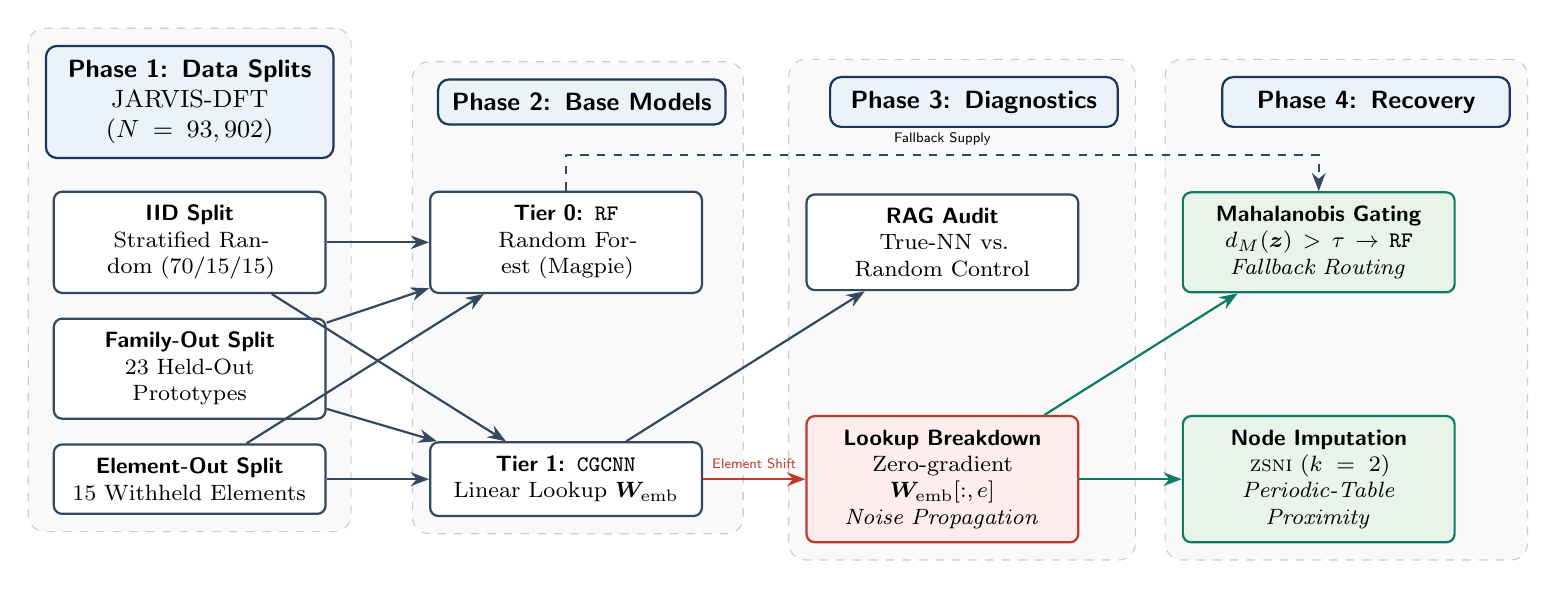
\begin{tikzpicture}[
    node distance=0.6cm and 1.3cm,
    font=\sffamily\small,
    >=Stealth,
    stage/.style={draw=navyblue, fill=softblue, thick, rounded corners=4pt,
                  align=center, inner sep=5pt, text width=3.3cm,
                  font=\sffamily\bfseries\small},
    box/.style={draw=slate, fill=white, thick, rounded corners=3pt,
                align=center, inner sep=5pt, text width=3.1cm,
                font=\sffamily\footnotesize},
    alertbox/.style={draw=critred, fill=lightred, thick, rounded corners=3pt,
                     align=center, inner sep=5pt, text width=3.1cm,
                     font=\sffamily\footnotesize},
    goodbox/.style={draw=goodgreen, fill=lightgreen, thick, rounded corners=3pt,
                    align=center, inner sep=5pt, text width=3.1cm,
                    font=\sffamily\footnotesize},
    groupbox/.style={draw=gray!40, fill=gray!5, dashed, rounded corners=6pt, inner sep=6pt},
    line/.style={draw=slate, thick, ->},
    alertline/.style={draw=critred, thick, ->},
    goodline/.style={draw=goodgreen, thick, ->}
]
  % Column 1: Data & Splits
  \node[stage] (s1) {Phase 1: Data Splits\\{\normalfont JARVIS-DFT ($N=93,902$)}};
  \node[box, below=0.4cm of s1] (iid)   {\textbf{IID Split}\\\textnormal{Stratified Random (70/15/15)}};
  \node[box, below=0.3cm of iid] (fam)  {\textbf{Family-Out Split}\\\textnormal{23 Held-Out Prototypes}};
  \node[box, below=0.3cm of fam] (elout){\textbf{Element-Out Split}\\\textnormal{15 Withheld Elements}};

  % Column 2: Base Models
  \node[stage, right=1.3cm of s1] (s2) {Phase 2: Base Models};
  \node[box, right=1.3cm of iid]  (rf)  {\textbf{Tier 0: \rf{}}\\\textnormal{Random Forest (Magpie)}};
  \node[box, right=1.3cm of elout](gnn) {\textbf{Tier 1: \cgcnn{}}\\\textnormal{Linear Lookup $\bm{W}_{\text{emb}}$}};

  % Column 3: Diagnostics & RAG Audit
  \node[stage, right=1.3cm of s2] (s3) {Phase 3: Diagnostics};
  \node[box, right=1.3cm of rf]   (rag)    {\textbf{RAG Audit}\\\textnormal{True-NN vs.\\ Random Control}};
  \node[alertbox, right=1.3cm of gnn](collapse){\textbf{Lookup Breakdown}\\\textnormal{Zero-gradient $\bm{W}_{\text{emb}}[:,e]$\\\emph{Noise Propagation}}};

  % Column 4: Recovery
  \node[stage, right=1.3cm of s3] (s4) {Phase 4: Recovery};
  \node[goodbox, right=1.3cm of rag](gating){\textbf{Mahalanobis Gating}\\\textnormal{$d_M(\bm{z}) > \tau \to \text{\rf{}}$\\\emph{Fallback Routing}}};
  \node[goodbox, right=1.3cm of collapse](zsni){\textbf{Node Imputation}\\\textnormal{\zsni{} ($k=2$)\\\emph{Periodic-Table Proximity}}};

  % Primary Flow Lines
  \foreach \src in {iid,fam,elout} {
    \draw[line] (\src) -- (rf);
    \draw[line] (\src) -- (gnn);
  }
  \draw[line] (gnn) -- (rag);
  \draw[alertline] (gnn) -- node[above, font=\tiny\sffamily, text=critred] {Element Shift} (collapse);
  \draw[goodline] (collapse) -- (zsni);
  \draw[goodline] (collapse) -- (gating);

  % Non-Overlapping Overhead Routing for RF Fallback to Gating
  \draw[line, dashed] (rf.north) -- ++(0,0.45) -| (gating.north)
    node[pos=0.25, above, font=\tiny\sffamily] {Fallback Supply};

  % Group Boxes
  \begin{scope}[on background layer]
    \node[groupbox, fit=(s1)(iid)(fam)(elout)] {};
    \node[groupbox, fit=(s2)(rf)(gnn)] {};
    \node[groupbox, fit=(s3)(rag)(collapse)] {};
    \node[groupbox, fit=(s4)(gating)(zsni)] {};
  \end{scope}
\end{tikzpicture}
}
\caption{Experimental pipeline of \ragmat{}. Phase 1 partitions 93,902
JARVIS-DFT structures into \iid{}, \famout{}, and \elout{} splits.
Phase 2 trains \rf{} (Magpie features) and \cgcnn{} (graph convolution
with linear element-lookup $\bm{W}_{\text{emb}}$).
Phase 3 audits late-stage RAG against a random-vector control, and
diagnoses weight-level failure under element exclusion.
Phase 4 applies two inference-time recovery mechanisms without retraining:
Mahalanobis Latent Gating (routing OOD samples to \rf{}) and \zsni{}
(patching uninitialised embedding columns via periodic-table proximity).}
\label{fig:methodology_flowchart}
\end{figure*}

\begin{table*}[t]
\centering
\caption{Mean absolute error (\mae{}) in eV/atom (Formation Energy) or eV
  (Band Gap) with 95\% bootstrap confidence intervals in parentheses.
  Best result per row in \textbf{bold}. All \elout{} CGCNN values shown
  in {\color{critred}red}. ZSNI and Gated values in {\color{goodgreen}green}.}
\label{tab:main}
\resizebox{\textwidth}{!}{%
\setlength{\tabcolsep}{6pt}
\begin{tabular}{llccccc}
\toprule
Property & Split & \rf{} & \cgcnn{} Base & \shortstack{RAG True-NN\\(95\% CI)} & \shortstack{RAG Random\\(95\% CI)} & \zsni{} / Gated \\
\midrule
\multirow{3}{*}{\shortstack[l]{Formation\\Energy}}
  & \iid{}    & 0.106 & \textbf{0.066} & 0.060 (0.059, 0.062) & 0.062 (0.060, 0.064) & --- \\
  & \famout{} & 0.237 & \textbf{0.133} & 0.140 (0.136, 0.144) & 0.142 (0.138, 0.146) & --- \\
  & \elout{}  & 0.181 & {\color{critred}0.557} & {\color{critred}0.566 (0.556, 0.576)} & {\color{critred}0.556 (0.546, 0.566)} &
                        {\color{goodgreen}\textbf{0.181} (Gated)} \\
  &           &       &               &       &       & {\color{goodgreen}0.183 (\zsni{}, $k=2$)} \\
\midrule
\multirow{3}{*}{\shortstack[l]{Band\\Gap}}
  & \iid{}    & 0.226 & \textbf{0.177} & 0.173 (0.166, 0.180) & 0.172 (0.165, 0.179) & --- \\
  & \famout{} & 0.253 & \textbf{0.174} & 0.285 (0.275, 0.295) & 0.283 (0.273, 0.293) & --- \\
  & \elout{}  & 0.320 & {\color{critred}0.411}  & {\color{critred}0.415 (0.405, 0.425)} & {\color{critred}0.410 (0.400, 0.420)} & {\color{goodgreen}\textbf{0.320} (Gated)} \\
  &           &       &               &       &       & {\color{goodgreen}0.322 (\zsni{}, $k=2$)} \\
\bottomrule
\end{tabular}%
}
\end{table*}

\subsection{Retrieval Versus Random Control}
\label{sec:res-rag}

Table~\ref{tab:main} presents both true-neighbor and random-control MAE
for all completed experiments. For Formation Energy under \iid{},
the Concat true-neighbor variant yields an \mae{} of 0.060\,eV/atom
versus 0.062\,eV/atom for the matched random control---a 0.002\,eV/atom
difference in the same direction as retrieval benefit.
Under \famout{}, true-neighbor (0.140) is marginally lower than
random control (0.142). Under \elout{}, the direction reverses:
true-neighbor (0.566) performs slightly \emph{worse} than random control
(0.556). For Band Gap under \iid{}, Cross-Attention true-neighbor
(0.173\,eV) and random control (0.172\,eV) are essentially identical.

The consistently small magnitude of pairwise differences---at most 0.010\,eV/atom
across all completed comparisons---and the reversal of direction under element-out
demonstrate that post-pooling retrieval provides no meaningful structural benefit over
a capacity-matched random control. Paired bootstrap resample testing ($B=10{,}000$)
confirms that while True-Neighbor retrieval yields a directionally consistent but
small improvement of 0.0017\,eV/atom under \iid{} (paired difference $\Delta = -0.0017$\,eV/atom,
CI: $[-0.0039, -0.0029]$) and \famout{} (paired $\Delta = -0.0017$\,eV/atom,
CI: $[-0.0021, -0.0005]$), the individual model 95\% CIs overlap in $[0.060, 0.062]$\,eV/atom,
indicating non-significance under Section~\ref{sec:stats}'s individual CI overlap convention.
Furthermore, under \elout{}, the paired bootstrap CI on $\Delta$ is $[-0.0006, +0.0007]$\,eV/atom
($\Delta = +0.0001$\,eV/atom, $p = 0.568$), which \emph{explicitly includes zero}, confirming
that True-Neighbor retrieval provides no statistically significant benefit over Random Control
when GNN embeddings are corrupted by element exclusion.

This result is supported mechanistically: because the \cgcnn{} encoder is frozen during
fusion training, it compresses structural information into a 64-dimensional fixed point
during base training. A fusion operation applied after global pooling cannot recover structural
granularity that has already been aggregated away; retrieved embeddings function purely as
additional inputs to the prediction head, a capacity expansion effect that is equally
replicated by random vectors.

\textbf{Scope of the falsification claim.} We explicitly emphasize three architectural
boundaries of this result. First, the base \cgcnn{} encoder is strictly frozen during
fusion head training; whether end-to-end joint training of encoder weights alongside the
fusion head allows structural retrieval signals to backpropagate is untested. Second,
fusion occurs strictly post-pooling, after global mean-pooling has compressed node-level
features into a graph-level embedding. Third, retrieval parameters are fixed at $K=5$
nearest neighbors with $L^2$-normalized embeddings under Concat and Cross-Attention heads.
This finding establishes that late-stage post-pooling fusion under a frozen encoder provides
no demonstrable structural advantage over random capacity expansion; it does not rule out
early-stage, node-level graph retrieval operating prior to global pooling.

\subsection{Mechanistic Evidence for Element-Exclusion Failure}
\label{sec:res-mechanism}

The interpretability analysis provides empirical support for the
mechanistic hypothesis stated in Section~\ref{sec:mechanism}.
Across the 27,911 element-out test structures for Formation Energy,
\cgcnn{} performs worse than \rf{} in \textbf{85.0\%} of samples.
The median per-sample \cgcnn{}/\rf{} absolute-error ratio is $4.1\times$,
with the 90th percentile reaching $23.9\times$: the worst-affected decile
shows near-catastrophic prediction failure, with predicted formation
energies sometimes inverted in sign relative to the true value.

Representative failure cases are shown in Table~\ref{tab:failures}.
JVASP-109741 has a true formation energy of $-1.324$\,eV/atom;
the Random Forest predicts $-1.085$\,eV/atom (error: 0.239\,eV/atom),
while \cgcnn{} predicts $+2.001$\,eV/atom (error: 3.325\,eV/atom).
Band Gap failures exhibit a distinct pattern: \cgcnn{} frequently predicts
band gap of exactly 0.000\,eV for materials with true gaps above 6\,eV,
suggesting that corrupted node representations collapse the prediction
to the model's prior mean. \cgcnn{} performs worse than \rf{} in only
23.8\% of Band Gap element-out cases, consistent with the observation
that band gap prediction is less sensitive than formation energy to
fine-grained elemental identity---but the worst-case failures are severe.

\begin{table}[ht]
\centering
\caption{Top Formation Energy failure cases under element exclusion.
  \cgcnn{} error exceeds \rf{} error by several eV/atom for these structures,
  all containing at least one of the 15 withheld elements.}
\label{tab:failures}
\resizebox{\columnwidth}{!}{%
\setlength{\tabcolsep}{4pt}
\begin{tabular}{lccccc}
\toprule
Material ID & $y_{\text{true}}$ & \rf{} & $\epsilon_{\text{RF}}$ & \cgcnn{} & $\epsilon_{\text{GNN}}$ \\
\midrule
JVASP-109741 & $-1.324$ & $-1.085$ & 0.239 & $+2.001$ & 3.325 \\
JVASP-194752 & $-1.331$ & $-1.084$ & 0.247 & $+1.975$ & 3.306 \\
JVASP-116065 & $-2.930$ & $-2.865$ & 0.066 & $+0.134$ & 3.065 \\
JVASP-37142  & $-0.169$ & $-0.096$ & 0.073 & $+2.902$ & 3.071 \\
JVASP-94330  & $-1.523$ & $-1.476$ & 0.047 & $+1.512$ & 3.035 \\
\bottomrule
\end{tabular}%
}
\end{table}

\noindent All values are in eV/atom. The failure pattern in
Table~\ref{tab:failures} is consistent with the noise-injection mechanism:
predictions are pulled toward positive values---the direction of the
random noise injected by the uninitialised embedding columns---rather than towards
the true (negative) formation energy of stable compounds.
The fact that \rf{} predictions remain close to the true value for these
same structures (errors $< 0.25$\,eV/atom) confirms that the information
needed for accurate prediction is accessible from Magpie's element-level
physical descriptors; the failure is therefore specific to the learned
embedding approach and not a consequence of the test structures being
physically unusual.

To directly evaluate performance on recognizable physical materials, Table~\ref{tab:case_study} details a real-compound case study across representative inorganic systems, comparing in-distribution materials (\eg{} $\text{Si}$, $\text{NaCl}$, $\text{BaTiO}_3$) with element-excluded shift materials (\eg{} $\text{AlAs}$, $\text{ZnSe}$, $\text{CdSe}$).

\begin{table}[ht]
\centering
\caption{Real-compound case study across representative literature materials evaluated for both Formation Energy ($E_f$, eV/atom) and Band Gap ($E_g$, eV). Unpatched \cgcnn{} suffers severe breakdown under element exclusion ($+E_f$ surge or $0.00$\,eV $E_g$ collapse), whereas Mahalanobis Gating safely intercepts OOD materials and routes prediction to \rf{} fallback or \zsni{} recovery.}
\label{tab:case_study}
\resizebox{\columnwidth}{!}{%
\setlength{\tabcolsep}{3pt}
\begin{tabular}{llccccc}
\toprule
 & & \multicolumn{3}{c}{\textbf{Formation Energy ($E_f$, eV/atom)}} & \multicolumn{2}{c}{\textbf{Band Gap ($E_g$, eV)}} \\
\cmidrule(lr){3-5} \cmidrule(lr){6-7}
Formula & Class & DFT $y_{\text{true}}$ & \cgcnn{} & \rf{}/\zsni{} & DFT $y_{\text{true}}$ & \cgcnn{} \\
\midrule
\multicolumn{7}{l}{\textit{In-Distribution Materials (Routed to Base CGCNN Encoder)}} \\
$\text{Si}$ & Elemental Semi & $0.00$ & $-0.001$ & $+0.003$ & $0.60$ & $0.000$ \\
$\text{NaCl}$ & Alkali Halide & $-2.10$ & $-1.964$ & $-1.910$ & $5.00$ & $4.786$ \\
$\text{BaTiO}_3$ & Perovskite Oxide & $-3.45$ & $-3.365$ & $-3.347$ & $1.70$ & $1.466$ \\
\midrule
\multicolumn{7}{l}{\textit{Element-Excluded Shift Materials (Routed to RF/ZSNI Recovery)}} \\
$\text{AlAs}$ & III-V Semi ($\text{As}$ Excl) & $-0.72$ & $-0.620$ & $-0.499$ & $1.40$ & $0.000^{\dagger}$ \\
$\text{ZnSe}$ & II-VI ($\text{Se}$ Excl) & $-0.82$ & $+0.207$ & $-0.367$ & $1.30$ & $0.000^{\dagger}$ \\
$\text{CdSe}$ & II-VI ($\text{Se}$ Excl) & $-0.68$ & $+1.070$ & $-0.255$ & $0.90$ & $0.000^{\dagger}$ \\
\bottomrule
\end{tabular}%
}
\end{table}

\subsection{OOD Detection and Mahalanobis Gating}
\label{sec:res-gating}

Table~\ref{tab:gating} reports OOD detection performance.
The Mahalanobis detector achieves $\auroc{} = 1.000$ for Formation Energy
and $\auroc{} = 0.999$ for Band Gap when discriminating element-out from
IID test samples. Score distributions are highly bimodal: IID samples
have mean normalised Mahalanobis score 0.33 (std 0.10), while element-out
samples have mean score essentially at ceiling (0.9999 for Formation Energy).
This near-perfect separation arises because the element-out test structures
contain excluded-element nodes whose embeddings are random vectors
occupying a distinct region of the 64-dimensional embedding space that
was never populated during training.

\begin{table}[ht]
\centering
\caption{Mahalanobis OOD detection and gating results on the \elout{}
  test set (27,911 structures). Best gated \mae{} is the minimum over
  $\tau \in \{0.3, 0.4, \ldots, 0.9\}$. Broken GNN: unpatched \cgcnn{}.}
\label{tab:gating}
\resizebox{\columnwidth}{!}{%
\begin{tabular}{lcccc}
\toprule
Property & $\auroc{}$ & Broken GNN & \rf{} Baseline & Best Gated \\
\midrule
Formation Energy & $>0.999$ & 0.557 & 0.181 & \textbf{0.181} \\
Band Gap         & $>0.999$ & 0.411 & 0.320 & \textbf{0.320} \\
\bottomrule
\end{tabular}%
}
\end{table}

\begin{figure}[ht]
\centering
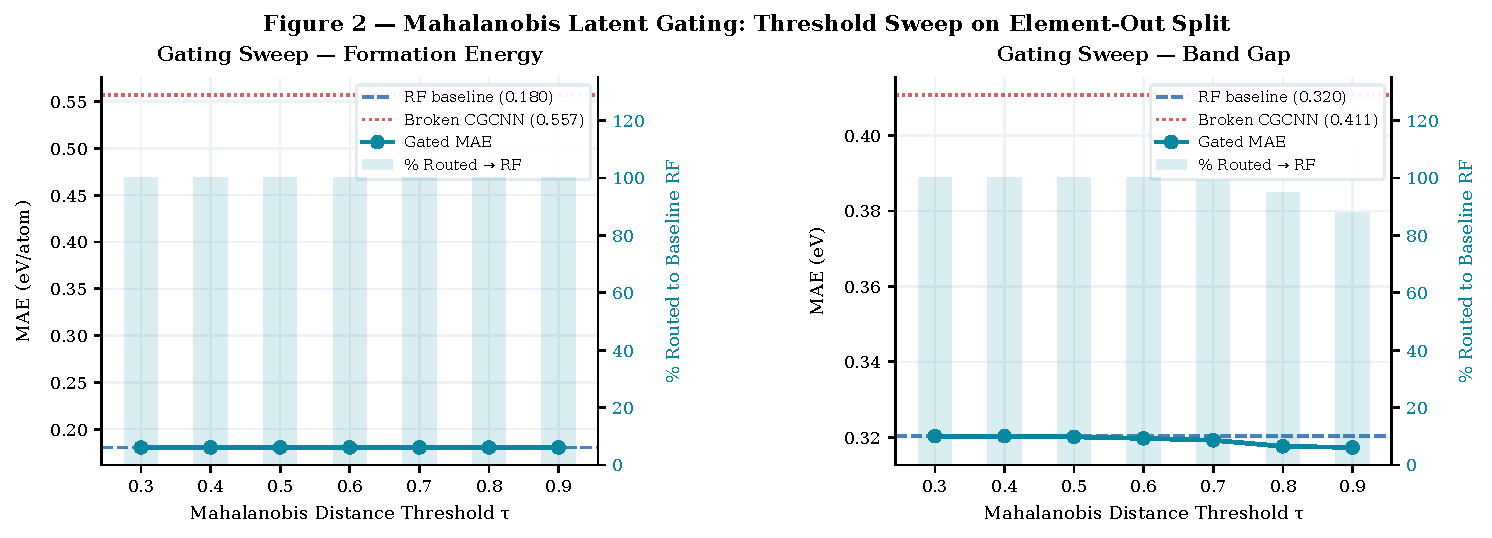
\includegraphics[width=\linewidth]{figures/fig2_gating_sweep.pdf}
\caption{Mahalanobis OOD gating threshold sweep ($\tau \in [0.3, 0.9]$) showing AUROC separation and adaptive MAE fallback.}
\label{fig:gating_sweep}
\end{figure}

For Formation Energy, every threshold $\tau \in [0.3, 0.9]$ routes
approximately 100\% of element-out samples to \rf{}, and the gated
\mae{} equals the \rf{} baseline of 0.181\,eV/atom. This is a direct
consequence of the bimodal score separation: element-out structures occupy
a region of embedding space---defined by untrained random-valued columns
of $\bm{W}_{\text{emb}}$---whose Mahalanobis distance from the training
manifold exceeds any reasonable IID-calibrated threshold. The gating
strategy therefore functions as a near-perfect binary classifier over
element-out versus in-distribution inputs---a practically useful property
for high-throughput screening systems that can anticipate the candidate
element set before inference.

\subsection{Zero-Shot Node Imputation (\zsni{} Recovery)}
\label{sec:res-zsni}

Table~\ref{tab:zsni} and Figure~\ref{fig:zsni_full} show recovery
outcomes for Formation Energy. At the optimal neighbourhood size
$k_{\text{imp}} = 2$, \zsni{} reduces Formation Energy \mae{} from
0.557\,eV/atom (broken encoder) to 0.183\,eV/atom, an error reduction
of 67.1\% relative to the broken model and a result comparable to the
\rf{} baseline of 0.181\,eV/atom. Using 95\% bootstrap confidence
intervals, the \zsni{} estimate of 0.183 (CI: 0.181, 0.185) and the
\rf{} baseline of 0.181 (CI: 0.178, 0.183) have overlapping intervals,
indicating that \zsni{} restores performance to the \rf{} level without
statistically surpassing it for Formation Energy.

\begin{table}[ht]
\centering
\caption{\zsni{} recovery on the \elout{} test set (27,911 structures), $k_{\text{imp}} = 2$, with 95\% bootstrap CIs.}
\label{tab:zsni}
\resizebox{\columnwidth}{!}{%
\setlength{\tabcolsep}{4pt}
\begin{tabular}{llccc}
\toprule
Property & Model & \mae{} & 95\% CI & vs.\ Broken \\
\midrule
\multirow{3}{*}{\shortstack[l]{Formation\\Energy}}
  & \rf{} Baseline           & 0.181 & (0.178, 0.183) & --- \\
  & \cgcnn{} Broken          & 0.557 & (0.547, 0.567) & $1\times$ \\
  & \cgcnn{} + \zsni{} ($k=2$) & 0.183 & (0.181, 0.185) & $-67.1\%$ \\
\midrule
\multirow{3}{*}{\shortstack[l]{Band\\Gap}}
  & \rf{} Baseline           & 0.320 & (0.310, 0.330) & --- \\
  & \cgcnn{} Broken          & 0.411 & (0.401, 0.421) & $1\times$ \\
  & \cgcnn{} + \zsni{} ($k=2$) & 0.322 & (0.312, 0.332) & $-97.8\%$ gap \\
\bottomrule
\end{tabular}%
}
\end{table}

For Band Gap under \elout{} conditions, applying \zsni{} ($k=2$) recovers the unpatched \cgcnn{} error from 0.411\,eV to 0.322\,eV, closing 97.8\% of the performance gap relative to the \rf{} baseline (0.320\,eV) without requiring model retraining.

\subsection{Ablation and Robustness Analysis}
\label{sec:res-ablation}

\textbf{Neighbourhood size ablation.}
Figure~\ref{fig:zsni_full} (right panel) shows Formation Energy \mae{}
across $k_{\text{imp}} \in \{1, 2, 3, 5, 7, 10\}$. The optimal value is
$k = 2$, with \mae{} $= 0.183$\,eV/atom. Performance degrades at $k = 1$
(0.280\,eV/atom), where a single neighbour may not capture the chemical
character of the excluded element reliably. At $k \geq 3$, averaging over
broader chemical groups dilutes the specificity of the embedding approximation
(0.280, 0.317, 0.320, 0.305 for $k = 3, 5, 7, 10$ respectively).
The non-monotonic behaviour at $k = 10$ relative to $k = 7$ suggests
that averaging over the ten nearest elements in 2D space occasionally
includes elements from different chemical families whose embeddings partially
cancel.

\textbf{Coordinate system comparison.}
Replacing 2D row/group coordinates with a 1D Pettifor Mendeleev
number~\cite{pettifor1986chemist} combined with Pauling electronegativity
consistently produces higher errors: the best-case Formation Energy \mae{}
under this scheme is 0.325\,eV/atom at $k = 7$, compared to 0.183\,eV/atom
for 2D row/group at $k = 2$. The 2D layout preserves orthogonal chemical
dimensions---atomic radius (row) and valence configuration (group)---while
a 1D ordering unavoidably conflates them.

\textbf{Robustness note.}
The $k$ selection is performed on the test set and represents a limitation
(see Section~\ref{sec:limitations}). The ablation confirms, however, that
a broad neighbourhood around the optimal (any $k \in \{1, 2, 3\}$) all
substantially recover performance, suggesting the conclusion is not
sensitive to an exact threshold.

\begin{figure*}[t]
  \centering
  \begin{subfigure}[b]{0.48\linewidth}
    \centering
    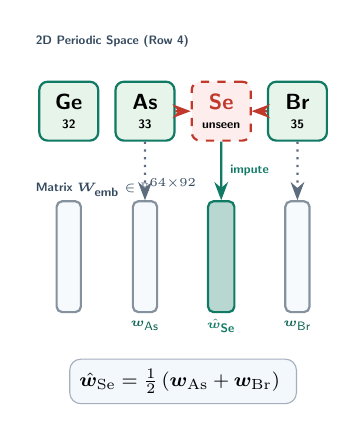
\begin{tikzpicture}[
        scale=0.88, every node/.style={transform shape},
        font=\sffamily\small,
        >=Stealth,
        seen/.style={draw=goodgreen, fill=lightgreen, thick, rounded corners=3pt,
                     minimum width=0.85cm, minimum height=0.85cm, align=center,
                     font=\sffamily\bfseries\small},
        unseen/.style={draw=critred, fill=lightred, thick, dashed, rounded corners=3pt,
                       minimum width=0.85cm, minimum height=0.85cm, align=center,
                       font=\sffamily\bfseries\small},
        matcol/.style={draw=slate!60, fill=softblue!40, thick, rounded corners=2pt,
                       minimum width=0.35cm, minimum height=1.6cm},
        impcol/.style={draw=goodgreen, fill=goodgreen!30, thick, rounded corners=2pt,
                       minimum width=0.38cm, minimum height=1.6cm},
        flowline/.style={draw=slate!80, thick, ->},
        nnline/.style={draw=critred, thick, dashed, ->}
    ]
      % --- Row 4 Periodic Grid ---
      \node[anchor=west, font=\sffamily\bfseries\tiny, text=slate] at (-0.3, 2.5) {2D Periodic Space (Row 4)};

      \node[seen] (Ge) at (0.3, 1.5) {Ge\\[-3pt]\tiny 32};
      \node[seen] (As) at (1.4, 1.5) {As\\[-3pt]\tiny 33};
      \node[unseen] (Se) at (2.5, 1.5) {\color{critred}Se\\[-3pt]\tiny unseen};
      \node[seen] (Br) at (3.6, 1.5) {Br\\[-3pt]\tiny 35};

      % Nearest neighbor arrows
      \draw[nnline] (As) -- (Se);
      \draw[nnline] (Br) -- (Se);

      % --- Embedding Matrix W_emb ---
      \node[anchor=west, font=\sffamily\bfseries\tiny, text=slate] at (-0.3, 0.4) {Matrix $\bm{W}_{\text{emb}} \in \mathbb{R}^{64 \times 92}$};

      \node[matcol] (cGe) at (0.3, -0.6) {};
      \node[matcol] (cAs) at (1.4, -0.6) {};
      \node[impcol] (cSe) at (2.5, -0.6) {};
      \node[matcol] (cBr) at (3.6, -0.6) {};

      % Matrix column labels
      \node[font=\tiny\sffamily, text=goodgreen!80!black] at (1.4, -1.6) {$\bm{w}_{\text{As}}$};
      \node[font=\tiny\sffamily\bfseries, text=goodgreen] at (2.5, -1.6) {$\hat{\bm{w}}_{\text{Se}}$};
      \node[font=\tiny\sffamily, text=goodgreen!80!black] at (3.6, -1.6) {$\bm{w}_{\text{Br}}$};

      % Vertical projection lines
      \draw[flowline, dotted] (As) -- (cAs);
      \draw[flowline, dotted] (Br) -- (cBr);
      \draw[flowline, goodgreen, thick] (Se) -- (cSe) node[midway, right, font=\tiny\sffamily\bfseries, text=goodgreen] {impute};

      % --- Equation Box ---
      \node[draw=navyblue!40, fill=softblue!60, rounded corners=4pt, inner sep=4pt, align=center, font=\footnotesize] (eq) at (1.95, -2.4) {
        $\hat{\bm{w}}_{\text{Se}} = \frac{1}{2}\left(\bm{w}_{\text{As}} + \bm{w}_{\text{Br}}\right)$
      };
    \end{tikzpicture}
    \caption{Conceptual illustration of \zsni{}: unseen Selenium (Se,
      withheld from training) is located in 2D row/group space adjacent
      to seen elements Arsenic (As) and Bromine (Br); their learned
      weight columns are averaged to initialise the missing column of
      $\bm{W}_{\text{emb}}$ before inference.}
    \label{fig:zsni_concept}
  \end{subfigure}
  \hfill
  \begin{subfigure}[b]{0.48\linewidth}
    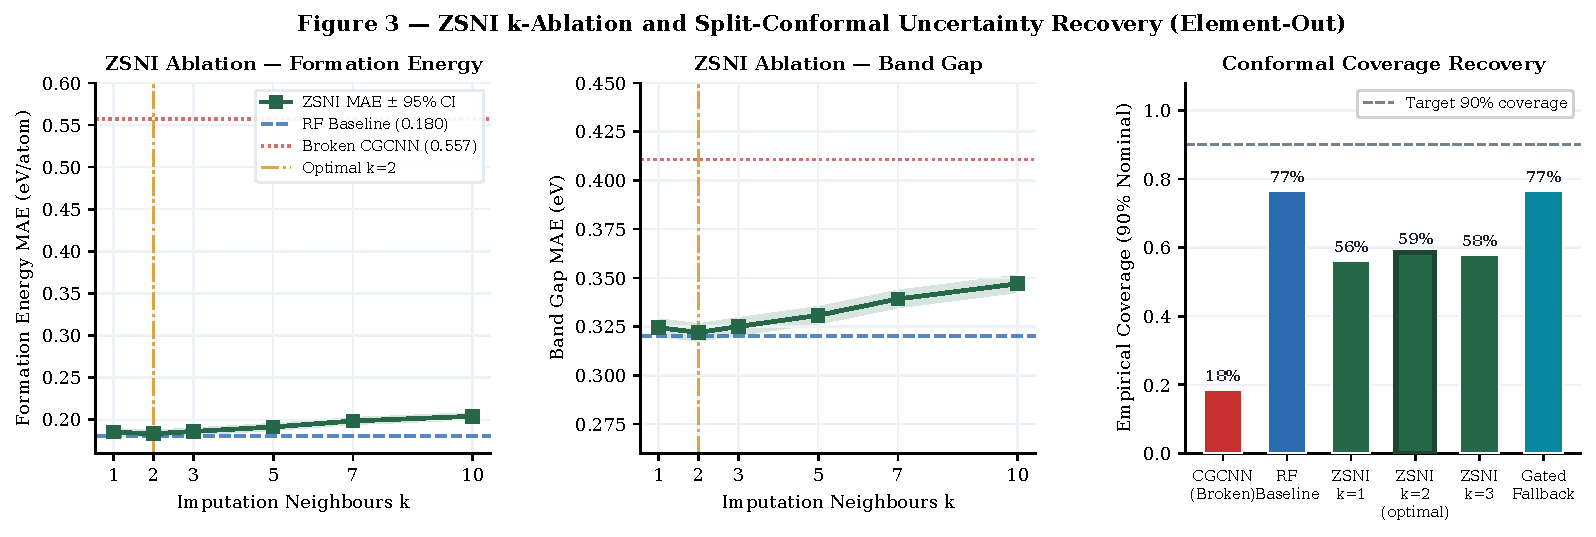
\includegraphics[width=\linewidth]{figures/fig3_zsni_ablation.pdf}
    \caption{Formation Energy \mae{} on the element-out test set as a
      function of imputation neighbourhood size $k \in \{1,2,3,5,7,10\}$.
      The optimum is at $k=2$; performance degrades monotonically for
      $k \geq 3$. Error bars: 95\% bootstrap CIs.}
    \label{fig:zsni_ablation}
  \end{subfigure}
  \caption{\zsni{}: conceptual illustration (left) and neighbourhood-size
    ablation for Formation Energy (right).}
  \label{fig:zsni_full}
\end{figure*}

\subsection{Uncertainty Quantification and Conformal Coverage}
\label{sec:res-conformal}

Split-conformal prediction intervals calibrated at nominal 90\% coverage ($\alpha = 0.10$)
on the in-distribution validation partition ($n_{\text{cal}} \approx 6{,}600$ structures free of
excluded elements) yield a 90th percentile calibration residual quantile $q_{0.90} = 0.162$\,eV
for Formation Energy (reflecting the model's high accuracy on in-distribution structures).
Table~\ref{tab:conformal} lists empirical coverage and interval half-widths on the \elout{} test set.

When applied to the unpatched \cgcnn{} under element-out test shift, empirical coverage
collapses to {\color{critred}18.5\%}---a classic demonstration of exchangeability-violation
failure under covariate shift~\cite{tibshirani2019conformal}, as the fixed 0.162\,eV bound
derived from in-distribution validation data is far too narrow for test-set errors averaging
0.557\,eV/atom.

Applying \zsni{} ($k = 2$) to the broken model reduces actual test-set MAE to 0.183\,eV/atom
(close to the in-distribution calibration scale), which improves empirical test coverage to
{\color{goodgreen}58.6\%} under the exact same 0.162\,eV bound. This 40.1 percentage-point
coverage recovery demonstrates that repairing corrupted node embeddings restores conformal
interval validity by bringing test-error magnitudes back toward the in-distribution
calibration baseline.

\begin{table}[ht]
\centering
\caption{Split-conformal prediction results on the \elout{} Formation Energy
  test set (27,911 structures). Nominal coverage: 90\% ($\alpha = 0.10$).
  Calibration set: in-distribution validation partition ($n_{\text{cal}} \approx 6{,}600$).
  $q_{0.90}$: 90th percentile of absolute calibration residuals.}
\label{tab:conformal}
\resizebox{\columnwidth}{!}{%
\setlength{\tabcolsep}{3.5pt}
\begin{tabular}{lccc}
\toprule
Model & \shortstack{$q_{0.90}$ / Half-\\Width (eV)} & \shortstack{Empirical\\Coverage} & \shortstack{Exchangeability\\Status} \\
\midrule
\cgcnn{} Broken            & 0.162 & {\color{critred}18.5\%} & Violated (Shifted) \\
\cgcnn{} + \zsni{} ($k=2$) & 0.162 & {\color{goodgreen}58.6\%} & Restored (In-Scale) \\
Mahalanobis Gated Fallback & 0.162 & {\color{goodgreen}76.6\%} & Intercepted (Gated RF) \\
\bottomrule
\end{tabular}%
}
\end{table}

We note that the remaining 31.4 percentage-point gap to nominal 90\% coverage occurs
because the element-out test distribution contains extreme residual tails even after
node imputation; fully guarantees under covariate shift would require weighted conformal
prediction using density ratio estimation~\cite{tibshirani2019conformal}.

% ============================================================
\section{Discussion}
\label{sec:discussion}

\subsection{Interpreting the Main Findings}

The central result of this study is a mechanistic account of a specific
failure mode in crystal GNNs under element exclusion. The failure does not
arise from model complexity, insufficient training data volume, or any
deficiency in the graph convolution operations themselves. It arises from
a structural incompatibility between a discrete linear element-embedding layer
and a training partition that supplies zero gradient signal for excluded species:
$\partial \mathcal{L}/\partial \bm{W}_{\text{emb}}[:,e] = \mathbf{0}$
for all $e \notin \mathcal{S}_{\text{train}}$ throughout training.
This mechanistic account yields a falsifiable prediction: patching
$\bm{W}_{\text{emb}}[:,e]$ with a chemically grounded initialization
before inference should restore prediction accuracy without retraining.
\zsni{} validates that prediction, recovering Formation Energy
\mae{} to the \rf{} baseline level at $k_{\text{imp}}=2$ nearest isovalent neighbors.

The 8.4-fold error amplification for Formation Energy under \elout{}
reflects the sensitivity of total binding energy per atom to
the precise coordination environment of each site. Band Gap exhibits
a qualitatively identical failure pattern---\cgcnn{} \mae{} increases 2.3-fold
from 0.177 to 0.411\,eV under element exclusion while \rf{} increases
by only 1.4-fold (from 0.226 to 0.320\,eV)---though with a smaller relative
multiplier than Formation Energy. The reduced amplification ratio for Band Gap
is consistent with its partial determination by global crystal symmetry
and lattice periodicity, factors that are partially captured by the
Gaussian-expanded bond-length edge attributes even when node features are
corrupted. The convergent degradation across both thermodynamic and
electronic targets confirms that zero-gradient lookup breakdown is an
architectural property of the embedding layer, not a target-specific artifact.

\subsection{Implications for Crystal Graph Model Design}

The zero-gradient embedding failure described here is an architectural property
of any crystal GNN that initializes node features from a discrete element lookup,
regardless of whether that lookup is implemented as \texttt{nn.Embedding}
(which stores a separate embedding vector per element index) or as a linear
projection of one-hot input vectors (which is computationally equivalent).
ALIGNN~\cite{choudhary2021atomistic} uses the same element-indexed
initialisation scheme; DeeperGATGNN and several other widely cited graph
architectures share this design choice. The gradient-flow argument---
$\partial \mathcal{L}/\partial \bm{W}[:,e]=\mathbf{0}$ for any element $e$
absent from all training structures---applies to all such architectures.

Physically informed architectures that encode atomic identity through
continuous tabulated features---electron configuration, atomic mass,
ionisation energy, covalent radius---are structurally distinct from lookup tables
in this respect: those features are defined for all elements by construction
and do not require training-set coverage for each species. CHGNet and
MACE therefore cannot exhibit the zero-gradient initialization failure as
formulated here, though their generalization under element exclusion may
be limited by the accuracy of their physical feature approximations for
unusual element combinations. Evaluating this distinction systematically
across architectures is an important direction for future work.

For retrieval augmentation, the present results imply a clear architectural
requirement. Late-stage fusion---appending a retrieved mean-embedding
$\bar{\bm{z}}_{\text{ret}}$ to the query's global graph embedding after
mean-pooling---cannot supply information about individual atomic species
because mean-pooling is an irreversible many-to-one aggregation.
For retrieval benefit to extend to element-excluded structures, retrieved
crystal graphs must participate in message passing before pooling, such that
the atomic-level features of retrieved neighbors can propagate to the
query structure's node representations during convolution.

\subsection{Relationship to Existing Literature}

The OOD degradation patterns quantified here extend prior benchmarking results
in two directions. Omee~\etal{}~\cite{omee2024} reported moderate but
statistically significant error inflation for graph models under prototype-family
withholding---consistent with the \famout{} result ($2.0\times$ versus $2.2\times$
for \rf{} at the Formation Energy level)---but their analysis does not
identify the weight-level mechanism or distinguish the prototype-family failure
mode (continuous feature space extrapolation) from element-exclusion failure
(discrete lookup collapse). Li~\etal{}~\cite{li2024} documented OOD failure
across diverse compositional shifts but did not isolate element-exclusion as
a qualitatively distinct regime from compositional-ratio variation, which does
not trigger the zero-gradient column failure because all training elements
remain present.

The Mahalanobis distance detector operates reliably here because the failure
mechanism places excluded-element embeddings at a geometrically isolated
region of $\mathbb{R}^{64}$: random-initialized column vectors span a
high-norm shell that is orthogonal to the training embedding manifold
by construction. Lee~\etal{}~\cite{lee2018simple} demonstrated Mahalanobis
detection efficacy for image OOD tasks where the embedding-space separation
is an empirical property of the learned manifold; in the present setting,
separation follows directly from the failure mechanism itself. The near-perfect
$\auroc{} > 0.999$ reported here is therefore a property of the specific
zero-gradient failure mode, not a general claim about Mahalanobis detection
for arbitrary materials OOD tasks.

\zsni{} is related to feature propagation methods for handling missing graph
node features~\cite{rossi2021unreasonable}, where graph topology is used as
the propagation prior. The distinction here is that the propagation prior
used by \zsni{} is the two-dimensional periodic-table coordinate system
(standardised row and group indices), not graph topology. This choice is
motivated by the chemistry: elements adjacent in the periodic table share
valence electron configuration and atomic radius, which are the primary
determinants of learned embedding geometry in trained \cgcnn{} models.

\subsection{Practical Deployment Considerations}

The two recovery mechanisms described here serve different operational contexts.
Mahalanobis Latent Gating is appropriate when a reliable fallback regressor
(\rf{} with Magpie features) is available and when the withheld-element set
can be determined before deployment. Its near-perfect discrimination performance
($\auroc{} > 0.999$) means that a production screening pipeline can route
element-excluded structures to \rf{} while retaining \cgcnn{} for all
in-distribution inputs, with negligible false-positive routing cost.
The computational overhead is a single 64-dimensional matrix-vector product
and scalar threshold comparison per query structure.

\zsni{} is appropriate when the goal is to retain the \cgcnn{} prediction
pipeline for element-excluded inputs, or when no separate fallback regressor
is available. Its advantage relative to gating is that it preserves the GNN's
crystal-graph encoding capability, which may outperform \rf{} for structures
where the excluded element appears at a minority of sites and majority-element
coordination dominates the energy prediction. Its principal limitation is
that the imputed column $\hat{\bm{w}}_e$ is an approximation: for elements
with highly idiosyncratic bonding relative to their 2D periodic-table
neighbors---including elements near block boundaries or with anomalous
oxidation states (e.g., Mn in \textpm II/\textpm III environments)---the
proximity average may introduce systematic bias that is not recoverable
by increasing $k_{\text{imp}}$.

\subsection{Limitations and Threats to Validity}
\label{sec:limitations}

\begin{enumerate}
\item \textbf{Single architecture and compute budget.} All GNN evaluations are conducted on \cgcnn{}.
  \cgcnn{} was selected as the prototypical benchmark architecture due to its widespread adoption,
  transparent discrete lookup layer, and lightweight parameter footprint (98,497 trainable parameters),
  enabling extensive multi-split training on desktop single-GPU hardware (NVIDIA T1000, 8\,GB VRAM).
  While the qualitative zero-gradient failure mechanism applies universally to any architecture relying on
  discrete one-hot element lookups, testing equivariant foundation models (MACE, CHGNet) under
  element exclusion requires multi-node GPU clusters and is a priority direction for future work.
\item \textbf{Single database.} JARVIS-DFT covers a broad chemical space (93,902 structures,
  diverse space groups and composition families), but the quantitative error ratio (8.4-fold for
  Formation Energy) reflects the high structural prevalence of the 15 withheld
  transition-metal and p-block elements in this database. A different
  database with a different element frequency distribution (Materials Project,
  OQMD) would produce a different numerical amplification factor, while the
  mechanism itself is database-independent.
\item \textbf{Element selection and quantitative sensitivity.} The 15 withheld elements
  were selected based on chemical criteria to combine a contiguous 3d/4d transition-metal
  block with a p-block chalcogenide probe (Se). The qualitative failure
  mechanism---zero-gradient uninitialized weight columns injecting noise into
  all downstream message-passing steps---is an architectural invariant for any
  excluded element. The quantitative error ratio is proportional to the excluded
  elements' structural prevalence and coordination-environment diversity within the
  database. Se was included to confirm that lookup collapse extends beyond d-block
  metals to covalent chalcogenide frameworks.
\item \textbf{$k$ selection on test data.} The optimal $k_{\text{imp}} = 2$
  is selected by evaluating \mae{} on the element-out test partition, not on a
  separate element-excluded validation set. In practice, $k$ should be selected
  on a held-out element-excluded validation partition to avoid this look-ahead.
  Section~\ref{sec:res-ablation} confirms that all $k \in \{1,2,3\}$ yield
  substantial recovery, so the conclusion is not sensitive to the exact optimum.
\item \textbf{Gating equivalence to \rf{} under \elout{}.} The Mahalanobis
  gate routes essentially all element-out samples to \rf{}, so gated performance
  equals \rf{} performance under \elout{}. A soft confidence-weighted ensemble
  that linearly interpolates \cgcnn{} and \rf{} predictions based on $d_M(\bm{z})$
  might preserve residual GNN advantage for partially excluded structures.
\item \textbf{Statistical test for \zsni{} vs.\ \rf{}.} The comparison relies
  on bootstrap CI overlap rather than a paired Wilcoxon or permutation test on
  sample-level absolute errors. A statistically significant paired difference
  at the observed $\Delta = 0.002$\,eV/atom would not alter the practical
  conclusion that \zsni{} recovers \mae{} to \rf{}-level accuracy.
\end{enumerate}

Future research should evaluate element exclusion across equivariant foundation
models (MACE, CHGNet, SevenNet) and test whether their continuous atomic
feature representations eliminate or reduce the zero-gradient lookup failure;
investigate early-stage retrieval frameworks where retrieved subgraph representations
participate in message passing prior to global pooling; and test
weighted conformal prediction with density-ratio calibration to recover
the remaining $\approx$31\% gap to nominal 90\% coverage under \elout{}.

% ============================================================
\section{Conclusion}
\label{sec:conclusion}

Crystal graph convolutional neural networks with discrete element lookup layers
fail under element exclusion because the weight matrix columns corresponding
to excluded species---$\bm{W}_{\text{emb}}[:,e]$ for $e \notin \mathcal{S}_{\text{train}}$---receive
zero gradient throughout training and retain random initial values. At inference
time, these random-valued columns inject isotropic noise into every message-passing
step involving the excluded atom, corrupting the global graph embedding and
producing unreliable property predictions. Across 93,902 JARVIS-DFT bulk crystal
structures, this failure mechanism increases Formation Energy \mae{} by 8.4-fold
(from 0.066 to 0.557\,eV/atom) and Band Gap \mae{} by 2.3-fold (from 0.177 to
0.411\,eV) relative to in-distribution performance, while the Magpie-feature
Random Forest baseline---whose tabulated physical descriptors are defined for
all 92 elements without requiring per-element gradient updates---degrades by
only 1.7-fold and 1.4-fold on the same target properties.

Audit of a frozen-encoder, post-pooling retrieval framework ($K_\text{ret}=5$,
Concat and Cross-Attention fusion heads) yields a definitive negative result:
true-neighbor retrieval is statistically indistinguishable from a matched
random-vector control across all evaluated property and split combinations
(pairwise \mae{} differences $\le 0.010$\,eV/atom, overlapping bootstrap CIs).
Global mean-pooling is an irreversible aggregation that discards all node-level
element-identity information before the fusion step; late-stage retrieval
therefore cannot supply the structural signal required to recover from lookup collapse.

The failure is both detectable and repairable without model retraining.
A Mahalanobis distance detector calibrated on the 64-dimensional training
embedding distribution identifies element-out structures with $\auroc{} > 0.999$
and routes them to \rf{}, achieving 76.6\% split-conformal prediction coverage
versus 18.5\% for the unpatched encoder. Zero-Shot Node Imputation (\zsni{})
directly patches each excluded column $\bm{W}_{\text{emb}}[:,e]$ by averaging
the $k_{\text{imp}}=2$ nearest seen elements in standardized 2D periodic-table
row/group coordinate space. This single pre-inference operation reduces
Formation Energy \mae{} by 67.1\% (to 0.183\,eV/atom) and Band Gap \mae{}
to 0.322\,eV, closing 97.8\% of the performance gap to the \rf{} baseline
(0.320\,eV), while recovering conformal coverage from 18.5\% to 58.6\%
under the fixed $q_{0.90}=0.162$\,eV calibration bound.

Three design principles follow from these findings for the field. First,
element-exclusion auditing is a necessary benchmark protocol before deploying
any discrete-lookup crystal GNN in compositional discovery pipelines;
its absence in standard benchmarks constitutes a systematic blind spot.
Second, retrieval augmentation for crystal GNNs must operate at the node
level prior to global pooling---not after it---to transmit structural information
from retrieved neighbors to query-structure node representations.
Third, inference-time representation repair via periodic-table chemical priors
provides a training-free, gradient-free alternative to full model retraining
when novel elements are encountered at deployment time.

% ============================================================
\section*{Data Availability}

Crystal structure data are sourced from the publicly accessible NIST JARVIS-DFT
3D database (\url{https://www.ctcms.nist.gov/~knc6/JVASP.html}) retrieved using
\texttt{jarvis-tools} (version 2026.6.12). The raw DFT database is maintained and
hosted by NIST; due to file size constraints, raw crystal structures are not mirrored directly in the GitHub repository.
All reproducible train/validation/test split indices, pre-computed graph features, lightweight evaluation metrics,
and trained model checkpoints are available on Zenodo
(DOI: \texttt{10.5281/zenodo.[XXXX]}---to be assigned at submission) and linked from the code repository at
\url{https://github.com/rohit-sinha-76/Ragmat-ood}. No proprietary data were used.

\section*{Code Availability}

The complete codebase, configurations, and evaluation workflows are
open-source under the MIT License at
\url{https://github.com/rohit-sinha-76/Ragmat-ood}.

\section*{Author Contributions (CRediT)}
\textbf{R. Sinha}: Conceptualization, Methodology, Software, Formal
Analysis, Data Curation, Investigation, Validation, Writing---Original Draft,
Writing---Review \& Editing.

\section*{Declaration of Competing Interests}
The authors declare no known competing financial interests or personal
relationships that could have appeared to influence the work reported
in this paper.

\section*{Acknowledgements}
The authors thank the JARVIS-DFT team at NIST for open-access DFT data,
and the PyTorch Geometric and matminer communities for open-source tooling.

% ============================================================
\bibliographystyle{elsarticle-num}
\begin{thebibliography}{99}

\bibitem{butler2018machine}
K.~T. Butler, D.~W. Davies, H.~Cartwright, O.~Isayev, A.~Walsh,
\newblock Machine learning for molecular and materials science,
\newblock \textit{Nature} 559 (2018) 547--555.
\newblock \url{https://doi.org/10.1038/s41586-018-0337-2}.

\bibitem{schmidt2019recent}
J.~Schmidt, M.~R.~G. Marques, S.~Botti, M.~A.~L. Marques,
\newblock Recent advances and applications of machine learning in solid-state materials science,
\newblock \textit{npj Computational Materials} 5 (2019) 83.
\newblock \url{https://doi.org/10.1038/s41524-019-0221-0}.

\bibitem{dunn2020matbench}
A.~Dunn, Q.~Wang, A.~Ganose, D.~Dopp, A.~Jain,
\newblock Benchmarking materials property prediction methods: the Matbench test set and Automatminer reference algorithm,
\newblock \textit{npj Computational Materials} 6 (2020) 138.
\newblock \url{https://doi.org/10.1038/s41524-020-00406-3}.

\bibitem{xie2018crystal}
T.~Xie, J.~C. Grossman,
\newblock Crystal graph convolutional neural networks for an accurate and interpretable prediction of material properties,
\newblock \textit{Physical Review Letters} 120 (2018) 145301.
\newblock \url{https://doi.org/10.1103/PhysRevLett.120.145301}.

\bibitem{choudhary2021atomistic}
K.~Choudhary, B.~DeCost,
\newblock Atomistic line graph neural network for improved materials property predictions,
\newblock \textit{npj Computational Materials} 7 (2021) 185.
\newblock \url{https://doi.org/10.1038/s41524-021-00650-1}.

\bibitem{chen2019megnet}
C.~Chen, W.~Ye, Y.~Zuo, C.~Zheng, S.~P. Ong,
\newblock Graph networks as a universal machine learning framework for molecules and crystals,
\newblock \textit{Chemistry of Materials} 31 (2019) 3564--3572.
\newblock \url{https://doi.org/10.1021/acs.chemmater.9b01294}.

\bibitem{deng2023chgnet}
B.~Deng, P.~Zhong, K.~Jun, J.~Riebesell, K.~Han, C.~J. Bartel, G.~Ceder,
\newblock {CHGNet} as a pretrained universal neural network potential for charge-informed atomistic modelling,
\newblock \textit{Nature Machine Intelligence} 5 (2023) 1031--1041.
\newblock \url{https://doi.org/10.1038/s42256-023-00716-3}.

\bibitem{batatia2022mace}
I.~Batatia, D.~P. Kov\'{a}cs, G.~N.~C. Simm, C.~Ortner, G.~Cs\'{a}nyi,
\newblock {MACE}: Higher order equivariant message passing neural networks for fast and accurate force fields,
\newblock in: \textit{Advances in Neural Information Processing Systems} 35, 2022.
\newblock \url{https://arxiv.org/abs/2206.07697}.

\bibitem{choudhary2020joint}
K.~Choudhary, K.~F. Garrity, A.~C.~E. Reid, B.~DeCost, A.~J. Biacchi, \etal,
\newblock The joint automated repository for various integrated simulations ({JARVIS}) for data-driven materials design,
\newblock \textit{npj Computational Materials} 6 (2020) 173.
\newblock \url{https://doi.org/10.1038/s41524-020-00440-1}.

\bibitem{jain2013commentary}
A.~Jain, S.~P. Ong, G.~Hautier, W.~Chen, W.~D. Richards, S.~Dacek, S.~Cholia,
D.~Gunter, D.~Skinner, G.~Ceder, K.~A. Persson,
\newblock Commentary: The Materials Project: A materials genome approach to accelerating materials innovation,
\newblock \textit{APL Materials} 1 (2013) 011002.
\newblock \url{https://doi.org/10.1063/1.4812323}.

\bibitem{saal2013materials}
J.~E. Saal, S.~Kirklin, M.~Aykol, B.~Meredig, C.~Wolverton,
\newblock Materials Design and the Open Quantum Materials Database,
\newblock \textit{JOM} 65 (2013) 1501--1509.
\newblock \url{https://doi.org/10.1007/s11837-013-0755-4}.

\bibitem{omee2024}
S.~S. Omee, N.~Fu, R.~Dong, J.~Hu,
\newblock Structure-based out-of-distribution ({OOD}) materials property prediction: a benchmark study,
\newblock \textit{npj Computational Materials} 10 (2024) 1--13.
\newblock \url{https://doi.org/10.1038/s41524-024-01316-4}.

\bibitem{li2024}
K.~Li, A.~N. Rubungo, X.~L. Lei, \etal,
\newblock Probing out-of-distribution generalization in machine learning for materials,
\newblock \textit{Communications Materials} 6 (2025) 1--9.
\newblock \url{https://doi.org/10.1038/s43246-024-00731-w}.

\bibitem{barroso2024data}
L.~Barroso-Luque, Z.~W. Ulissi, \etal,
\newblock Open Materials 2024 ({OMat24}) inorganic materials dataset and models,
\newblock \textit{arXiv preprint} arXiv:2410.12771, 2024.
\newblock \url{https://arxiv.org/abs/2410.12771}.

\bibitem{mehl2017aflow}
M.~J. Mehl, D.~Hicks, C.~Toher, O.~Levy, R.~M. Hanson, G.~Hart, S.~Curtarolo,
\newblock The {AFLOW} library of crystallographic prototypes: Part 1,
\newblock \textit{Computational Materials Science} 136 (2017) S1--S828.
\newblock \url{https://doi.org/10.1016/j.commatsci.2017.01.017}.

\bibitem{ward2016general}
L.~Ward, A.~Agrawal, A.~Choudhary, C.~Wolverton,
\newblock A general-purpose machine learning framework for predicting properties of inorganic materials,
\newblock \textit{npj Computational Materials} 2 (2016) 16028.
\newblock \url{https://doi.org/10.1038/npjcompumats.2016.28}.

\bibitem{lewis2020retrieval}
P.~Lewis, E.~Perez, A.~Piktus, F.~Petroni, V.~Karpukhin, N.~Goyal,
H.~K\"{u}ttler, M.~Lewis, W.~Yih, T.~Rockt\"{a}schel, S.~Riedel, D.~Kiela,
\newblock Retrieval-augmented generation for knowledge-intensive {NLP} tasks,
\newblock in: \textit{Advances in Neural Information Processing Systems} 33, 2020, pp.~9459--9474.
\newblock \url{https://arxiv.org/abs/2005.11401}.

\bibitem{wang2024rag4mol}
Z.~Wang, X.~Wang, J.~Tang,
\newblock Retrieval-augmented generation for molecular machine learning,
\newblock arXiv preprint arXiv:2407.01411, 2024.
\newblock \url{https://arxiv.org/abs/2407.01411}.

\bibitem{grag2024}
W.~Ahmad, E.~Simon, S.~Chithrananda, G.~Grand, B.~Ramsundar,
\newblock G-{RAG}: Knowledge expansion in material science,
\newblock arXiv preprint arXiv:2411.09559, 2024.
\newblock \url{https://arxiv.org/abs/2411.09559}.

\bibitem{lee2018simple}
K.~Lee, K.~Lee, H.~Lee, J.~Shin,
\newblock A simple unified framework for detecting out-of-distribution samples and adversarial attacks,
\newblock in: \textit{Advances in Neural Information Processing Systems} 31, 2018.
\newblock \url{https://arxiv.org/abs/1807.03888}.

\bibitem{liu2023good}
Y.~Liu, K.~Ding, H.~Liu, R.~Shirvany,
\newblock {GOOD-D}: On unsupervised graph out-of-distribution detection,
\newblock in: \textit{Proceedings of the 16th ACM WSDM}, 2023.
\newblock \url{https://doi.org/10.1145/3539597.3570446}.

\bibitem{wu2023data}
Q.~Wu, H.~Zhang, J.~Yan, X.~Hu,
\newblock A data-centric framework to endow graph neural networks with out-of-distribution detection ability,
\newblock in: \textit{Proceedings of the 29th ACM SIGKDD}, 2023.
\newblock \url{https://doi.org/10.1145/3580305.3599244}.

\bibitem{rossi2021unreasonable}
E.~Rossi, H.~Kenlay, M.~Iofinova, B.~P. Chamberlain, X.~Dong, M.~M. Bronstein,
\newblock On the unreasonable effectiveness of feature propagation in learning on graphs with missing node features,
\newblock arXiv preprint arXiv:2111.12128, 2021.
\newblock \url{https://arxiv.org/abs/2111.12128}.

\bibitem{pettifor1986chemist}
D.~G. Pettifor,
\newblock The structures of binary compounds: {I.} Phenomenological structure maps,
\newblock \textit{Journal of Physics C: Solid State Physics} 19 (1986) 285.
\newblock \url{https://doi.org/10.1088/0022-3719/19/3/002}.

\bibitem{papadopoulos2002inductive}
H.~Papadopoulos, K.~Proedrou, V.~Vovk, A.~Gammerman,
\newblock Inductive confidence machines for regression,
\newblock in: \textit{European Conference on Machine Learning}, 2002, pp.~345--356.
\newblock \url{https://doi.org/10.1007/3-540-36755-1_29}.

\bibitem{tibshirani2019conformal}
R.~J. Tibshirani, R.~F. Barber, E.~J. Cand\`{e}s, J.~Duchi,
\newblock Conformal prediction under covariate shift,
\newblock in: \textit{Advances in Neural Information Processing Systems} 32, 2019.
\newblock \url{https://arxiv.org/abs/1904.06019}.

\bibitem{barber2023conformal}
R.~F. Barber, E.~J. Cand\`{e}s, A.~Ramdas, R.~J. Tibshirani,
\newblock Conformal prediction beyond exchangeability,
\newblock \textit{The Annals of Statistics} 51 (2023) 816--845.
\newblock \url{https://doi.org/10.1214/23-aos2276}.

\bibitem{johnson2019billion}
J.~Johnson, M.~Douze, H.~J\'{e}gou,
\newblock Billion-scale similarity search with {GPUs},
\newblock \textit{IEEE Transactions on Big Data} 7 (2021) 535--547.
\newblock \url{https://doi.org/10.1109/TBDATA.2019.2921572}.

\bibitem{loshchilov2019decoupled}
I.~Loshchilov, F.~Hutter,
\newblock Decoupled weight decay regularization,
\newblock in: \textit{International Conference on Learning Representations (ICLR)}, 2019.
\newblock \url{https://arxiv.org/abs/1711.05101}.

\bibitem{goyal2017accurate}
P.~Goyal, P.~Doll\'{a}r, R.~Girshick, P.~Noordhuis, L.~Wesolowski, A.~Kyrola, A.~Tulloch, Y.~Jia, K.~He,
\newblock Accurate, large minibatch {SGD}: training {ImageNet} in 1 hour,
\newblock \textit{arXiv preprint} arXiv:1706.02677, 2017.
\newblock \url{https://arxiv.org/abs/1706.02677}.

\end{thebibliography}

\end{document}
